\chapter{Continuo tridimensionale}


\section{Il problema elastico}\label{PEla}
Consideriamo un corpo che in una configurazione di riferimento occupa la regione $\Omega$. 
La frontiera $\partial\Omega$ è data dall'unione di due sottoinsiemi disgiunti $\partial_N\Omega$ e $\partial_D\Omega$, con $\partial\Omega=\partial_N\Omega\cup\partial_D\Omega$, $\partial_N\Omega\cap\partial_D\Omega=\emptyset$.
Sulla parte del bordo $\partial_N\Omega$ sono applicate delle forze di superficie, mentre su $\partial_D\Omega$ è prescritto uno spostamento $\bar{\ub}$. Definiamo \textit{stato elastico} la l'insieme dei campi $\{ \ub, \Eb, \Tb\}$, la determinazione del quale rappresenta la soluzione del \textit{problema elastico}
\begin{definition}
	\begin{equation}
	\begin{cases}
	\Div\mathbf{T}+\mathbf{b}=\mathbf{0}&\mathrm{in~}\Omega,\\
		\mathbf{T}=\mathbf{T}^\top&\mathrm{in~}\Omega,\\
		\mathbf{T}\mathbf{n}=\mathbf{s}&\mathrm{su~}\partial_{N}\Omega,\\
		\mathbf{T}=\mathbb{C}\mathbf{E}&\mathrm{in~}\Omega,\\
		\mathbf{E}=\mathbf{E}(\mathbf{u})=\frac{1}{2}(\nabla\mathbf{u}+\nabla\mathbf{u}^\top)&\mathrm{in~}\Omega,\\
		\mathbf{u}=\bar{\mathbf{u}}&\mathrm{su~}\partial_{D}\Omega,
		\end{cases}
\end{equation}
\end{definition}
Le prime tre equazioni sono le \textit{equazioni di equilibrio}, la quarta è l’equazione costitutiva, la quinta è l’equazione di compatibilità che assicura che il tensore della deformazione  $\Eb$ sia congruente con lo spostamento $\ub$, e l’ultima impone che tale spostamento sia uguale a quello prescritto su $\partial_{D}\Omega$. Se, come di solito, il tensore di elasticità $\Co$ mappa tensori simmetrici in simmetrici, la seconda equazione (la simmetria di $\Tb$) diventa superflua.

Se le incognite sono gli elementi dello stato elastico, i dati del problema sono: la configurazione di riferimento $\Omega$,  il tensore di elasticità $\Co$, le forze di volume $\bb$, le forze di superficie $\sb$ e la regione $\partial_{N}\Omega$ su cui sono applicate, lo spostamento $\bar{\ub}$ e la regione $\partial_{D}\Omega$ su cui è impresso.

\subsection{Unicità della soluzione}
Denotiamo con $\Dc =\{\bb, \sb, \bar{\ub}\}$ un insieme di dati (forze di volume, di superficie e spostamenti al bordo) per il problema elastico \eqref{PEla}, cui corrisponda 
uno stato elastico $\Sc=\{ \ub, \Eb, \Tb\}$. Dati due insiemi $\Dc^{1}=\{\bb^1, \sb^1, \bar{\ub}^1\}$ e $\Dc^2=\{\bb^2, \sb^2, \bar{\ub}^2\}$ e due conseguenti stati elastici
$\Sc^1=\{ \ub^1, \Eb^1, \Tb^1\}$, $\Sc^2=\{ \ub^2, \Eb^2, \Tb^2\}$, si ha che vale il teorema di \textit{sovrapposizione degli effetti}: 
\begin{equation}
\textrm{i dati}\quad\alpha^1\Dc^1+\alpha^2\Dc^2 \qquad \textrm{provocano lo stato elastico}\quad \alpha^1\Sc^1+\alpha^2\Sc^2.
\end{equation}
 In altri termini, la soluzione del problema elastico corrispondente alla combinazione lineare
di due carichi è uguale alla combinazione lineare delle soluzioni corrispondenti ai due carichi.
La dimostrazione è banale: occorre verificare infatti tutte le equazioni del problema \eqref{PEla}, che sono tutte lineari; ad esempio:
$\Div \Tb^1+\bb^1=\mathbf{0}$ e $\Div \Tb^2+\bb^2=\mathbf{0}$ implicano che
\begin{equation}
\Div(\alpha^1\Tb^1+\alpha^2\Tb^2)+(\alpha^1\bb^1+\alpha^2\bb^2)=\alpha^1(\Tb^1+\bb^1)+\alpha^2(\Tb^2+\bb^2);
\end{equation}
in maniera analoga si verificano tutte le altre.

Possiamo a questo punto enunciare il \textit{Teorema di unicità di Kirchhoff}:
\begin{definition}
Sia $\Co$ definito positivo. Se $\Sc^1$ e $\Sc^2$ sono due stati elastici del problema elastico \eqref{PEla}, allora
\begin{equation}
\Eb^1=\Eb^2, \qquad \Tb^1=\Tb^2, \qquad \ub^1=\ub^2+\rb,
\end{equation}
dove $\rb$ è uno spostamento rigido infinitesimo.
\end{definition}
In altri termini la soluzione del problema elastico (se esiste) è \textit{unica}, a meno di uno spostamento rigido.

Dimostriamo il teorema. Immaginiamo che ad una stessa condizione di carico $\Dc$ corrispondano due stati elastici $\Sc^1$ e $\Sc^2$. Se indichiamo con
\begin{equation}
\Delta \Sc=\Sc^2-\Sc^1=\{\ub, \Eb, \Tb\}
\end{equation}
lo stato elastico differenza, questo sarà allora causato da una condizione di carico nulla $\Delta\Dc=\emptyset$, per la sovrapposizione degli effetti. Pertanto l'energia totale 
immagazzinata sarà nulla:
\begin{equation}
\int_{\Omega}\frac{1}{2}\Co \Eb \cdot \Eb=0,
\end{equation}
Poiché $\Co$ è definito positivo, questo è possibile se e solo se 
\begin{equation}
\Eb=\mathbf{0}  \qquad \Longrightarrow\qquad \Eb^1=\Eb^2.
\end{equation}
Ne segue immediatamente che 
\begin{equation}
\Tb=\mathbf{0} \qquad \Longrightarrow\qquad \Tb^1=\Tb^2.
\end{equation}
Poiché lo spostamento $\ub$ è rigido infinitesimo se e solo se $\Eb(\ub)=\mathbf{0}$, segue che
\begin{equation}
\ub^2=\ub^1+\rb.
\end{equation}




\subsection{Formulazione in spostamenti: l'equazione di Navier}
Ci sono vari modi di affrontare il problema elastico. È possibile determinare un insieme di equazioni in cui l'unica incognita sia il campo di spostamento $\ub$, utilizzando l'equazione costitutiva e la relazione tra spostamento e deformazione. In particolare, il problema elastico può essere riformulato così:
\begin{equation}
	\begin{cases}
		\mathrm{Trovare~}\mathbf{u}:\mathbf{u}=\bar{\mathbf{u}}\mathrm{~su~}\partial_D\Omega\mathrm{~e}\\
		\begin{cases}
			\begin{aligned}
				&\mathrm{~div}(\mathbb{C}\mathbf{E}(\mathbf{u}))+\mathbf{b}=\mathbf{0}  \quad &&\mathrm{~in~}\Omega,\\
			&[\mathbb{C}\mathbf{E}(\mathbf{u})]\mathbf{n}=\mathbf{s} &&\mathrm{~su~}\partial_N\Omega.
			\end{aligned}
	\end{cases}
		\end{cases}
\end{equation}

Utilizzando per $\Co \Eb$ l'espressione per i materiali isotropi \eqref{const3D}, si ha che
\begin{equation}
\Tb= \frac{E}{1+\nu}\left(\frac12(\nabla\ub+\nabla\ub^\top) +\frac{\nu}{1-2\nu}(\operatorname{tr}\nabla\ub)\,\Ib\right);
\end{equation}
per determinarne la divergenza osserviamo che
\begin{equation}
\Div \nabla\ub =\Delta \ub \qquad (\Delta \ub)_i=u_{i,jj}
\end{equation}
dove $\Delta(\cdot)$ è l'operatore laplaciano e 
\begin{equation}
\Div (\nabla \ub^\top)=\nabla \Div \ub, \qquad \Div\big(( \operatorname{tr}\nabla\ub)\,\Ib\big)=\Div(\Div \ub \,\Ib)=\nabla \Div \ub.
\end{equation}
Infatti
\begin{equation}
(\Div \nabla\ub^\top)_i)=(\nabla\ub^\top)_{ij,j}=u_{j,ji}=(\Div \ub),_i=\Big(\nabla (\Div \ub)\Big)_i
\end{equation}
e
\begin{equation}
\Div(\Div \ub \,\Ib)=(\Div \ub)\Div \Ib+\nabla\Div \ub=\nabla\Div \ub.
\end{equation}

Mettendo insieme questi risultati,  il problema diventa
\begin{definition}
	\begin{equation}\label{eqNav}
	\begin{cases}
		\mathrm{Trovare~}\mathbf{u}:\mathbf{u}=\bar{\mathbf{u}}\mathrm{~su~}\partial_D\Omega\mathrm{~e}\\
		\begin{cases}
			\begin{aligned}
				&\Delta \ub +\frac{1}{1-2\nu}\nabla \Div \ub+\frac{\bb}{G}=\mathbf{0}  \quad &&\mathrm{~in~}\Omega,\\
				&\frac{E}{1+\nu}{\left(\frac12(\nabla \ub +\nabla \ub^\top)+\frac{\nu}{1-2\nu}(\Div \ub)\mathbf{I}\right)}\mathbf{n}=\mathbf{s} &&\mathrm{~su~}\partial_N\Omega.
			\end{aligned}
		\end{cases}
	\end{cases}
\end{equation}
\end{definition}
La \eqref{eqNav}$_1$ è detta \textit{equazione di Navier}.


\subsection{Formulazione in sforzi: l'equazione di Beltrami-Michell}
In caso di assegnazione della sola trazione al bordo $\sb$, può convenire scegliere il tensore degli sforzi $\Tb$, piuttosto che lo spostamento. Così facendo però occorre garantire che alla deformazione $\Eb=\Co^{-1}\Tb$ corrisponda un campo di spostamento $\ub$ tale che $\Co^{-1}\Tb=\frac12 (\nabla \ub+\nabla \ub ^\top)$, con $\ub=\bar{\ub}$ su $\partial_D \Omega$.

%\subsubsection{La condizione di compatibilità}
%Dato un arbitrario campo di deformazione $\Eb$, la relazione tra spostamento e deformazione
%\begin{equation}
%	\Eb=\frac12(\nabla\ub +\nabla\ub^\top)
%\end{equation}
%costituisce un'equazione differenziale  lineare del primo ordine nel campo di spostamento $\ub$, la cui soluzione non è garantita esistere. Mostreremo che una condizione \textit{necessaria} per l'esistenza di soluzioni è che il campo di deformazione soddisfi una certa condizione di compatibilità, che è anche \textit{sufficiente} a garantire l'esistenza se il dominio è semplicemente connesso.
%
%Per prima cosa osserviamo che il campo di deformazione $\Eb$ e il vettore della rotazione infinitesima $\wb$ soddisfano la seguente condizione:
%\begin{equation}\label{RotE}
%	\Rot \Eb=\nabla \wb.
%\end{equation}
%%Ricordiamo che le componenti del rotore di un vettore $\vb$ sono 
%%\begin{equation}
%%(\Rot \vb)_i=	\epsilon_{ijk}v_{k,j}
%%\end{equation}
%%dove
%%\begin{equation}
%%\epsilon_{ijk}=\eb_i\times\eb_j\cdot\eb_k
%%\end{equation}
%%è il simbolo di Ricci (v. \eqref{Ricci}).
%%, tale che 
%%\begin{equation}\epsilon_{ijk}=\begin{cases}+1&\text{se tutti gli indici $i,j,k$ sono diversi e la loro sequenza}\\&\text{ è una permutazione di classe pari di $1,2,3$};\\0&\text{se almeno due degli indici $i, j, k$ sono uguali;}\\-1&\text{se tutti gli indici  $i,j,k$ sono diversi e la loro sequenza}\\&\text{è una permutazione di classe dispari di $1,2,3$}\end{cases}
%%\end{equation}
%%Dato un campo tensoriale $\Ab$ il suo rotore è così definito:
%%\begin{equation}
%%(\Rot \Ab)\ab \coloneqq \Rot(\Ab^\top \ab), \qquad \forall \ab \in \Vc;
%%\end{equation}
%%in componenti:
%%\begin{equation}
%%	(\Rot\Ab)_{ij}=\epsilon_{ipq}A_{jq},_{p}.
%%\end{equation}
%Per dimostrare la \eqref{RotE}, calcoliamo il rotore del gradiente dello spostamento (v. \eqref{RotT}):
%\begin{equation}
%	(\Rot(\nabla\ub))_{ij}=\epsilon_{ipq}(\nabla\ub)_{jq,p}=\epsilon_{ipq}(u_{j,q}),p=\epsilon_{ipq}u_{j,qp}=0;
%\end{equation}
%inoltre si ha che 
%\begin{equation}
%	(\Rot(\nabla\ub^\top))_{ij}=\epsilon_{ipq}(u_{q,j}),_p=\epsilon_{ipq}u_{q,jp}=(\epsilon_{ipq}u_{q,p}),_j=2 w_{i,j}=2 (\nabla \wb)_{ij}.
%\end{equation}
%Nell'ultima uguaglianza si è introdotto il vettore
%\begin{equation}
%	\wb \coloneqq \frac12 \Rot \ub;
%\end{equation}
%poiché, facendo uso della \eqref{epsdel}, possiamo scrivere la seguente successione di eguaglianze,
%\begin{equation}
%	\begin{aligned}
%		(\wb \times \ab)_i &=\epsilon_{ijk}w_j a_k=\frac12\epsilon_{ijk}\epsilon_{jpq}u_{q,p}a_k=-\frac12\epsilon_{jik}\epsilon_{jpq}u_{q,p}a_k=-\frac{1}{2}(\delta_{ip}\delta_{kq}-\delta_{iq}\delta_{kp})u_{q,p}a_k\\
%		&=\frac12 (u_{i,k}-u_{k,i})a_k=\frac{1}{2}(\nabla \ub-\nabla \ub^\top)_{ik}a_k=W_{ik}a_k=(\Wb \ab)_i,
%	\end{aligned}
%\end{equation}
%per ogni $\ab$, possiamo identificare $\wb$ con l'assiale del tensore della rotazione infinitesima $\Wb$, sicché
%\begin{equation}
%	\Wb \ab=\frac{1}{2}\Rot \ub \times \ab.
%\end{equation}
%
%
%Concludiamo allora che 
%\begin{equation}
%	\Rot \Eb =\frac12\big( \Rot (\nabla \ub) + \Rot (\nabla \ub^\top)=\nabla \wb.
%\end{equation}
%Applicando nuovamente l'operatore di rotore alla \eqref{RotE}, arriviamo alla conclusione che una condizione necessaria per l'esistenza di un campo di spostamento è che $\Eb$ soddisfi la seguente \textit{condizione di compatibilità}:
%\begin{definition}
%	\begin{equation}\label{RotRot}
%		\Rot \Rot \Eb =\mathbf{0}.
%	\end{equation}
%\end{definition}
%
%
%Dimostriamo adesso che la condizione \eqref{RotRot}, non è solo sufficiente, ma anche necessaria, se il dominio è semplicemente connesso; in altre parole, se $\Rot \Rot \Eb=\mathbf{0}$, allora certamente esiste un campo vettoriale $\ub$ tale che $\Eb =\sym \nabla \ub$.
%
%Per dimostrarlo ci servono due risultati  preparatori:
%\begin{enumerate}
%	\item Sia $\Tb\in \Lin$ tale che $\Rot \Tb =\mathbf{0}$, allora esiste un campo vettoriale $\ub$ tale che\footnote{Per dimostrarlo, consideriamo i vettori
%		\begin{equation}
%			\ab_i =\Tb^\top \eb_i,
%		\end{equation}
%		dove $\eb_i$ sono i vettori della base; si ha che
%		\begin{equation}
%			\Rot \ab_i= \Rot (\Tb^\top \eb_i)=\Rot(\Tb^\top)\eb_i=0
%		\end{equation}
%		e dunque esistono dei campi scalari $u_i$ tali che $\ab_i=\nabla u_i$.
%		%
%		Definiamo $\ub \coloneqq u_i \eb_i$; allora
%		\begin{equation}
%			\ab_i=\nabla u_i =\nabla(\ub \cdot \eb_i)=(\nabla \ub)^\top\eb_i=\Tb ^\top \eb_i,
%		\end{equation}
%		da cui deduciamo \eqref{Tnabu}.}
%	\begin{equation}\label{Tnabu}
%		\Tb=\nabla \ub.
%	\end{equation}
%	\item Sia $\Tb \in \Lin$ tale che $\Rot \Tb=\mathbf{0}$ e $\operatorname{tr}\Tb=0$, allora esiste $\Wb \in \Skw$ tale che\footnote{
%		Dimostriamolo: sia $\ub$ il vettore definito nella nota precedente e $\Wb$ il tensore antisimmetrico associato a $-\ub$. Allora
%		\begin{equation}
%			\Div \ub = \operatorname{tr}\nabla \ub =\operatorname{tr}\Tb =0.
%		\end{equation}
%		In  virtù della \eqref{identitadiff}$_9$
%		\begin{equation}
%			-\Rot \Wb =(\Div \ub)\Ib-\nabla \ub=-\nabla \ub =-\Tb,
%		\end{equation}
%		da cui il risultato.
%	}
%	\begin{equation}
%		\Tb=\Rot \Wb.
%	\end{equation}
%\end{enumerate}
%
%Torniamo dunque alla dimostrazione che, se $\Rot \Rot \Eb=\mathbf{0}$, allora  esiste un campo vettoriale $\ub$ tale che $\Eb =\sym \nabla \ub$. Assumiamo che $\Rot\Rot\Eb=\mathbf{0}$ in $\Omega$.  Sia $\Ab =\Rot \Eb$; poiché $\Eb \in \Sym$, 
%\eqref{identitadiff}$_8$ implica che
%\begin{equation}
%	\operatorname{tr}\Ab=0.
%\end{equation}
%Poiché $\Rot \Ab=\mathbf{0}$, allora esiste un campo tensoriale $\Wb\in\Skw$ tale che
%\begin{equation}
%	\Ab =-\Rot \Wb.
%\end{equation}
%Visto che $\Ab =\Rot \Eb$,
%\begin{equation}
%	\Rot (\Eb+ \Wb)=\mathbf{0};
%\end{equation}
%esiste allora un campo vettoriale $\ub$ tale che
%\begin{equation}
%	\Eb+ \Wb= \nabla \ub.
%\end{equation}
%Prendendo la parte simmetrica dell'ultima uguaglianza, concludiamo allora che esiste $\ub$ tale che
%\begin{equation}
%	\Eb = \sym \nabla \ub.
%\end{equation}
%
%
%\vspace{.3cm}

%\subsubsection{L'equazione di Beltrami-Michell}

 Per farlo, occorre utilizzare una condizione di compatibilità \eqref{RotRot} che, utilizzando il legame costitutivo, può essere allora riscritta come
\begin{equation}
\Rot \Rot \Eb =\Rot \Rot \Co^{-1}\Tb=\mathbf{0}.
\end{equation}
Il problema elastico può allora  essere così formulato:
\begin{equation}
	\begin{cases}
		\mathrm{Trovare~}\mathbf{T}:\\
		\begin{cases}
			\begin{aligned}
					&\Div\Tb +\bb=\mathbf{0} \quad &&\mathrm{~in~}\Omega,\\
				&\Rot \Rot \Co^{-1}\Tb=\mathbf{0}&& \mathrm{~in~}\Omega,\\
				&\Tb\nb =\sb &&\mathrm{~su~}\partial_N\Omega.
			\end{aligned}
		\end{cases}
	\end{cases}
\end{equation}

 Se si ipotizza il materiale isotropo, la  \eqref{costinv} consente di scrivere la seguente condizione su $\Tb$:
 \begin{equation}
 \Rot \Rot \Tb -\frac{\nu}{1+\nu}\Rot \Rot \big( (\operatorname{tr}\Tb)\,\Ib\big)=\mathbf{0}.
 \end{equation}
%Utilizzando l'identità
%\begin{equation}
%	\begin{aligned}
%			\Rot \Rot \Ab=-\Delta \Ab-\nabla(\nabla(\operatorname{tr}\Ab))+\nabla(\Div \Ab)+(\nabla(\Div\Ab))^\top+(\Delta(\operatorname{tr}\Ab)-\Div(\Div\Ab))\Ib,\end{aligned}
%\end{equation}
 Con un  po' di fatica e facendo anche uso dell'equazione di equilibrio, si trova 
 \begin{equation}\label{BeltrM}
 	\Delta \Tb +\frac{1}{1+\nu}\nabla \nabla (\operatorname{tr}\Tb)+\nabla \bb+\nabla \bb^\top+\frac{\nu}{1-\nu}(\Div \bb) \Ib =\mathbf{0},
  \end{equation}
 detta equazione di \textit{Beltrami-Michell}.
 %Per proseguire, osserviamo che ogni tensore simmetrico $\Ab$ sufficientemente regolare soddisfa la seguente identità differenziale:
%\begin{equation}
%	\begin{aligned}
%		\Rot \Rot \Ab=-\Delta \Ab-\nabla(\nabla(\operatorname{tr}\Ab))+\nabla(\Div \Ab)+(\nabla(\Div\Ab))^\top+(\Delta(\operatorname{tr}\Ab)-\Div(\Div\Ab))\Ib.\end{aligned}
%\end{equation}
%Di conseguenza
%\begin{equation}
%\operatorname{tr}(\Rot \Rot \Ab)=\Delta(\operatorname{tr}\Ab)-\Div \Div \Ab;
%\end{equation}
%inoltre, per $\Ab=\alpha \Ib$, si ha
%\begin{equation}
%\Rot \Rot (\alpha \Ib)=(\Delta \alpha)\Ib-\nabla \nabla \alpha,
%\end{equation}
%e quindi, in particolare
%\begin{equation}
%\operatorname{tr}\big(\Rot\Rot (\alpha\Ib)\big)=2\Delta \alpha.
%\end{equation}

%Per poter assegnare $\bar{\ub}$ su $\partial_D\Omega$, occorre esprimerlo in termini di sforzo. Sappiamo che
%\begin{equation}
%\sb =\Tb \nb =
%\end{equation}

Il problema di trazione  nel caso isotropo dunque può così essere formulato:
\begin{definition}
	\begin{equation}
		\begin{cases}
			\mathrm{Trovare~}\mathbf{T}:\\
			\begin{cases}
				\begin{aligned}
					&\Div\Tb +\bb=\mathbf{0} \quad &&\mathrm{~in~}\Omega,\\
					&\Delta \Tb +\frac{1}{1+\nu}\nabla \nabla (\operatorname{tr}\Tb)+\nabla \bb+\nabla \bb^\top+\frac{\nu}{1-\nu}(\Div \bb) \Ib =\mathbf{0}, \quad &&\mathrm{~in~}\Omega,\\
					&\Tb \nb=\mathbf{s} &&\mathrm{~su~}\partial_N\Omega.
				\end{aligned}
			\end{cases}
		\end{cases}
	\end{equation}
\end{definition}

Per dimostrare l'equazione di Beltrami-Michell conviene lavorare per componenti.
Partiamo dalla condizione di compatibilità \eqref{RotRot} scritta in componenti:
\begin{equation}\label{rotrotcomp}
	E_{ij,kl} + E_{kl,ij} - E_{ik,jl} - E_{jl,ik} = 0;
\end{equation}
L'equazione costitutiva inversa \eqref{costinv} in componenti è
\begin{equation}\label{constinvcomp}
	E_{ij} = \frac{1+\nu}{E} T_{ij} - \frac{\nu}{E} \delta_{ij} \Theta, \qquad 	\Theta \coloneqq \operatorname{tr} \Tb.
\end{equation}


Inserendo la \eqref{constinvcomp} nella \eqref{rotrotcomp} otteniamo
\begin{equation}\label{rotrotcompT}
	T_{ij,kl} + T_{kl,ij} - T_{ik,jl} - T_{jl,ik} = \frac{\nu}{1+\nu} \left( \delta_{ij} \Theta_{,kl} + \delta_{kl} \Theta_{,ij} - \delta_{ik} \Theta_{,jl} - \delta_{jl} \Theta_{,ik} \right).
\end{equation}

Poniamo $l = k$, ottenendo
\begin{equation}
	T_{ij,kk} + T_{kk,ij} - T_{ik,jk} - T_{jk,ik} = \frac{\nu}{1+\nu} \left( \delta_{ij} \Theta_{,kk} + \delta_{kk} \Theta_{,ij} - \delta_{ik} \Theta_{,jk} - \delta_{jk} \Theta_{,ik} \right),
\end{equation}
oppure, più semplicemente,
\begin{equation}
	\Delta T_{ij} + \Theta_{,ij} - T_{ik,jk} - T_{jk,ik} = \frac{\nu}{1+\nu} \left( \delta_{ij} \Delta \Theta + 3 \Theta_{,ij} - 2 \Theta_{,ij} \right).
\end{equation}

Dalle equazioni di equilibrio otteniamo
\begin{equation}
	T_{pq,q} + b_p = 0 \quad \Rightarrow \quad T_{pq,qr} = -b_{p,r},
\end{equation}
e quindi
\begin{equation}
	\Delta T_{ij} + \frac{1}{1+\nu} \Theta_{,ij} - \frac{\nu}{1+\nu} \delta_{ij} \Delta \Theta = -(b_{i,j} + b_{j,i}).
\end{equation}

Questo è un sistema di 9 equazioni, ma solo 6 sono indipendenti, per via delle simmetrie degli indici $i$ e $j$, quindi questa combinazione lineare delle 6 equazioni originali è equivalente a queste ultime.

Ora dobbiamo esprimere $\Theta$ in termini di $b_{ij}$. A questo scopo, poniamo $k = i$ e $l = j$ nella \eqref{rotrotcompT} e sommiamo rispetto agli indici ripetuti, ottenendo:
\begin{equation}
	2 T_{ij,ij} - T_{ii,jj} - T_{jj,ii} = \frac{\nu}{1+\nu} \left( 2 \delta_{ij} \Theta_{,ij} - \delta_{ii} \Theta_{,jj} - \delta_{jj} \Theta_{,ii} \right);
\end{equation}
poiché $T_{ii} = T_{jj} = \Theta$,
\begin{equation}
	\delta_{ij} \Theta_{,ij} = \Theta_{,ii} = \Delta \Theta, \quad \delta_{ii} \Theta_{,jj} = 3 \Delta \Theta,
\end{equation}
otteniamo
\begin{equation}
	T_{ij,ij} = \frac{1-\nu}{1+\nu} \Delta \Theta.
\end{equation}
Osserviamo adesso che 
\begin{equation}
	T_{ij,ij} = -b_{j,j} = -\Div \bb,
	\end{equation}
e quindi
\begin{equation}
	\Delta \Theta = -\frac{1+\nu}{1-\nu} \Div \bb,
\end{equation}
da cui finalmente otteniamo
\begin{equation}
\Delta T_{ij}+\frac{1}{1+\nu}\, \Theta_{i,j}+\frac{\nu}{1-\nu}\delta_{ij}\, \Div \bb+(b_{i,j}+b_{j,i})=0,
\end{equation}
che corrisponde alla \eqref{BeltrM}.


\subsection{Soluzioni generali delle equazioni di equilibrio}
In assenza di forze di volume le equazioni di equilibrio prendono la forma
\begin{equation}
\Div \Tb =\mathbf{0}, \qquad \Tb =\Tb^\top.
\end{equation}

Se $\Ab$ è un campo tensoriale su $\Omega$ e se $\Lc$ è un operatore differenziale con valori che sono campi tensoriali simmetrici, allora
\begin{equation}
	\Tb =\Lc (\Ab)
\end{equation}
sarà una soluzione delle equazioni di equilibrio se 
\begin{equation}
	\Div \Lc(\Ab)=\mathbf{0}.
\end{equation}
Un campo di $\Ab$ con queste proprietà è detto \textit{funzione di sforzo}. La prima soluzione delle equazioni di equilibrio è dovuta a \textsc{Airy} (1863), nel caso bidimensionale. Le generalizzazioni al caso 3D furono ottenute da \textsc{Maxwell} (1868) e \textsc{Morera} (1892). Nel 1821 \textsc{Beltrami} osservò che le soluzioni di Maxwell e Morera possono essere considerate come un caso particolare di quella che viene denominata \textit{soluzione di Beltrami}:

\begin{definition}
Sia $\Ab$ un campo tensoriale simmetrico sufficientemente regolare e sia
\begin{equation}
\Tb =\Rot \Rot \Ab
\end{equation}
Allora 
\begin{equation}
\Div \Tb =\mathbf{0}, \quad \Tb=\Tb^\top.
\end{equation}
\end{definition}

La dimostrazione si basa sulle due seguenti identità:
\begin{equation}
\Div \Rot \Ab =\Rot \Div \Ab^\top, \qquad \Div(\Rot \Ab)^\top=\mathbf{0}.
\end{equation}

In un sistema di riferimento cartesiano, la soluzione di Beltrami ha la forma
\begin{equation}
T_{ij}=\epsilon_{imn}\epsilon_{jpq}A_{mp,nq}.
\end{equation}


\begin{remark}
È possibile dimostrare che la soluzione di Beltrami non è completa, nel senso che non tutti i campi di sforzo $\Tb$ sono rappresentabili come $\Rot \Rot \Ab$. In particolare, i campi di sforzo che non sono \textit{auto-equilibrati} non possono essere rappresentati tramite la soluzione di Beltrami. Una soluzione completa può essere rappresenta nella forma di \textit{Beltrami-Schaefer}:
\begin{definition}
	Sia $\Ab$ un campo tensoriale simmetrico sufficientemente regolare e $\hb$ un campo vettoriale armonico, e sia
	\begin{equation}
		\Tb = \Rot \Rot \Ab +2 \sym \nabla \hb -(\Div \hb)\,\Ib.
	\end{equation}
	Allora
	\begin{equation}
		\Div \Tb= \mathbf{0}, \qquad \Tb =\Tb^\top.
	\end{equation}
\end{definition}
\end{remark}



Se ci si limita al caso piano e alla soluzione di Beltrami, il tensore $\Ab$ ha tutte le componenti nulle tranne una, sicché
%\begin{equation}
%[\Ab]=\left[\begin{array}{ccc}
%0	& 0 & 0 \\
%0	& 0 &  0\\
%0	&0  & \varphi
%\end{array}\right]
%\end{equation}
\begin{equation}
	\Ab=\varphi\,\eb_3\otimes\eb_3
\end{equation}
e dunque
\begin{equation}\label{Airy}
T_{11}=\varphi,_{22}, \qquad T_{22}=\varphi,_{11}, \quad T_{12}=-\varphi,_{12}.
\end{equation}
La funzione $\varphi$ è detta \textit{funzione di Airy}.

In assenza di forze di volume, la condizione di compatibilità diventa 
\begin{equation}
\Delta \Tb +\frac{1}{1+\nu}\nabla \nabla (\operatorname{tr}\Tb)=\mathbf{0}.
\end{equation}
Moltiplicando scalarmente per $\Ib$ (ovvero prendendo la traccia della precedente relazione), si ottiene la condizione che
\begin{equation}\label{trharm}
\Delta (\operatorname{tr}\Tb)=\mathbf{0},
\end{equation}
ovvero la traccia del tensore di sforzo deve essere armonica. Se si usa per $\Tb$ la rappresentazione di Airy, si ottiene allora che
\begin{equation}\label{biharmonic} 
\Delta \Delta \varphi=0.
\end{equation}

Dunque, nel caso piano, il problema elastico può essere risolto tramite la ricerca di una funzione di sforzo $\varphi$, che deve essere biarmonica, e che soddisfi le opportune condizioni al bordo.


Storicamente, il problema a valori al bordo per la funzione di Airy è stato risolto con un metodo semi-inverso, assegnando un \textit{Ansatz} per $\varphi$, spesso dettato dalla forma del dato al bordo. Lo svantaggio di questo modo di procedere euristico risiede nel fatto che serve una certa esperienza per comprendere il particolare tipo di soluzione che si adatta al problema in esame, che comunque non garantisce il successo dell'impresa. 



\subsection{Problemi in coordinate cartesiane}
Se lavoriamo in un sistema di riferimento cartesiano,  dalla \eqref{biharmonic} segue che qualunque polinomio in $x_1$, $x_2$ di grado inferiore a quattro è biarmonico ed è dunque adatto ad essere selezionato come funzione di Airy.  Si consideri adesso un polinomio di grado $n$
\begin{equation}
	P_n(x_1,x_2)=a_0x_1^n+a_1 x_1^{n-1}x_2+a_2x_1^{n-1}x_2^2+\ldots+a_nx_2^n=\sum_{i=0}^na_i\,x_1^{n-i}x_2^i,
\end{equation}
parametrizzato da $(n+1)$ coefficienti indipendenti $a_i$ $(i=0,\ldots,n)$. Sostituendo l'espressione di $P_n(x_1,x_2)$ in \eqref{biharmonic}, giacché ogni termine è differenziato 4 volte, si ottiene un nuovo polinomio di grado $(n-4)$:
\begin{equation}\label{qn}
	q_{n-4}(x_1,x_2):=\nabla\nabla p_n(x_1,x_2)=\sum_{i=0}^{n-4}b_i\,x_1^{n-4-i}x_2^i.
\end{equation}
Gli $(n-3)$ coefficienti $b_0,\ldots b_{n-4}$ si ottengono facilmente uguagliando i coefficienti dei due membri dell'equazione \eqref{qn}. Per esempio, si ottiene 
\begin{equation}
	b_0=n(n-1)(n-2)(n-3)a_0+4(n-2)(n-3)a_2+24a_4.
\end{equation}
La funzione $p_n(x_1,x_2)$ è dunque armonica se e soltanto se $q_{n-4}(x_1,x_2)$ è nulla per ogni valore di $x_1$ e $x_2$, ovvero se ogni termine della serie \eqref{qn} è identicamente nullo e dunque se $b_i=0$ $(i=0,\ldots n-4)$. Le $(n-3)$ equazioni risultanti sono dunque vincoli sui coeffcienti $a_i$.


\vspace{.5cm}

\noindent\textsf{\small\textit{\textbf{Trazione assiale}}}


Consideriamo un dominio rettangolare $\Omega$ di base $2b$ e altezza $2h$ soggetto ad una trazione $p$ ad entrambi gli estremi. Fissiamo il sistema di riferimento nel baricentro del rettangolo. 

Le condizioni al bordo da soddisfare sono:
\begin{equation}\label{uniaxialbc}
	\begin{aligned}
		&T_{11}=p, \quad T_{12}=0, \quad {\rm in}\; \pm b \\
		&T_{22}=0, \quad T_{12}=0, \quad {\rm in}\; \pm h.
	\end{aligned}
\end{equation}

Volendo adoperare il metodo delle tensioni ricerchiamo  un campo di sforzo autoequilibrato. Data la simmetria del problema, siamo indotti a cercare campi di sforzo aventi la seguente forma:
\begin{equation}
	\Tb=\widehat\Tb(x_1)=T_{11}(x_1)\,\eb_1\otimes\eb_1.
\end{equation}
La condizione di equilibrio locale richiede
\begin{equation}
	\Div\Tb=T_{11,1}\, \eb_1 =\mathbf{0}, \quad \Rightarrow\quad T_{11}=\sigma_0,
\end{equation}
dove $\sigma_0$ è una costante. Gli infiniti campi di sforzo equilibrati hanno dunque rappresentazione generale
\begin{equation}
	\Tb=\sigma_0\,\eb_1\otimes \eb_1.
\end{equation}
La condizione al bordo \eqref{uniaxialbc}$_1$ costringe la costante $\sigma_0$ ad essere uguale a $p$.
Si osserva che la condizione di compatibilità \eqref{trharm} è identicamente soddisfatta per qualsiasi campo equilibrato. 
%In questo senso il problema è `isostatico', prescindendo la soluzione da questioni di compatibilità.

Volendo adoperare la rappresentazione di Airy, giacché le condizioni riguardano sforzi costanti sul bordo, siamo portati a cercare una funzione  della forma
\begin{equation}
	\varphi=c_{02}x_2^2,
\end{equation}
che fornisce i seguenti campi di sforzo:
\begin{equation}
T_{11}=2c_{02}, \quad T_{22}=T_{12}=0.
\end{equation}
La prima delle condizioni \eqref{uniaxialbc} implica che $c_{02}=p/2$, mentre le altre sono identicamente soddisfatte. Gli sforzi sono dunque
\begin{equation}
T_{11}=p, \quad T_{22}=T_{12}=0.
\end{equation}


\vspace{.5cm}

\noindent\textsf{\small\textit{\textbf{Taglio puro}}}

Consideriamo un dominio quadrato di lato $2a$ soggetto ad una forza di taglio $\tau$ sulle sue facce.  Le condizioni al bordo da soddisfare sono
\begin{equation}
	\begin{aligned}
		&T_{11}=0, \quad T_{12}=\tau, \quad {\rm in}\; \pm a \\
		& T_{22}=0, \quad T_{12}=\tau, \quad {\rm in}\; \pm a.
	\end{aligned}
\end{equation}
Vista la simmetria del problema, cerchiamo  campi di sforzo aventi la seguente forma:
\begin{equation}
	\Tb=\widehat\Tb(x_1)=T_{12}(x_1,x_2)\,\big(\eb_1\otimes\eb_2+\eb_2\otimes\eb_1\big).
\end{equation}
La condizione di equilibrio locale richiede
\begin{equation}
	\Div\Tb=T_{12,2}\,\eb_1+T_{12,1}\,\eb_2=\mathbf{0}, \quad \Longrightarrow T_{12}(x_1, x_2)=\tau_0,
\end{equation}
dove $\tau_0$ è una costante. Ancora una volta, la compatibilità è garantita. Il valore di $\tau_0$, è determinato dalle condizioni al bordo: $\tau_0=\tau$.

Volendo adoperare la funzione di Airy, scegliamo
\begin{equation}
	\varphi=c_{11}x_1x_2,
\end{equation}
che fornisce i seguenti campi di sforzo:
\begin{equation}
	T_{11}=T_{22}=0, \quad T_{12}=-c_{11}.
\end{equation}
Di nuovo, le condizioni al bordo determinano la costante $c_{11}=-\tau$.



\vspace{.5cm}

\noindent\textsf{\small\textit{\textbf{Flessione pura}}}

Il rettangolo in Fig. \eqref{fig:bending} è soggetto a due coppie di intensità $M$ applicate alle estremità.

Le condizioni al bordo da soddisfare sono:
\begin{equation}\label{bendingbc}
	\begin{aligned}
		&T_{22}=0, \quad T_{12}=0 \quad &&{\rm in}\; x_2=\pm a, \\
		&T_{12}=0, \quad \int_{-a}^{a}T_{11}{\rm d}x_2=0, \quad \int_{-a}^{a}x_2T_{11}{\rm d}x_2=M \quad &&{\rm in}\; x_1=\pm b.
	\end{aligned}
\end{equation}
Le condizioni al bordo sulle facce $x_2=\pm b$ sono state rilassate e scritte in forma debole. 

Date le condizioni di simmetria, questa volta scegliamo
\begin{equation}
	\Tb=\widehat{\Tb}(x_1,x_2)=T_{11}(x_1,x_2)\,\eb_1\otimes\eb_1.
\end{equation}
La richiesta che il tensore di sforzo sia a divergenza nulla implica che
\begin{equation}
T_{11,1}=0, \quad \Longrightarrow \quad T_{11}(x_1,x_2)=\widehat{T}_{11}(x_2).
\end{equation}
Il campi di sforzo equilibrati si riducono quindi ad una famiglia di campi tensoriali parametrizzati da una funzione scalare della sola coordinata  $x_2$. Tra questi, i compatibili sono quelli la cui traccia è armonica:
\begin{equation}
	\Delta(\Tr\Tb)=\widehat{T}_{11,22}(x_2)=0, \qquad \Longrightarrow \qquad \widehat{T}_{11,22}(x_2)=c_1+c_2x_2.
\end{equation}
Le costanti $c_i$ ($i=1,2$) sono determinate dalle condizioni al bordo:
\begin{equation}
	\begin{aligned}
		& 0=\int_{-a}^{a}T_{11}=\int_{-a}^{a}(c_1+c_2x_2)=2c_1a,\\
		& M=\int_{-a}^{a}T_{11}=\int_{-a}^{a}(c_1x_2+c_2x_2^2)=\frac{2}{3}a^3c_2,
	\end{aligned}
\end{equation}
che porgono
$$
a_1=0, \quad a_2=\frac{3M}{2a^3}.
$$

Volendo affrontare il problema usando la funzione di Airy, occorre considerare che la coppia $M$ agli estremi è staticamente equivalente ad una tensione normale al bordo lineare. Scegliamo dunque
\begin{equation}
	\varphi=c_{03}x_2^3,
\end{equation}
da cui
\begin{equation}
	T_{11}=6c_{03}x_2, \quad T_{22}=T_{12}=0.
\end{equation}
La condizione \eqref{bendingbc}$_5$ implica che $c_{03}=M/4a^3$, mentre le altre sono automaticamente soddisfatte. Gli sforzi risultano dunque:
\begin{equation}
	T_{11}=\frac{3M}{2a^3}x_2, \quad T_{22}=	T_{12}=0.
\end{equation}
Confrontiamo il risultato ottenuto con le predizioni della teoria della trave. Assumendo che il pannello sia una trave rettangolare con spessore  costante, il momento di inerzia risulta essere $I=2/3a^3$. Dalla teoria di De Saint Venant, si sa che
\begin{equation}
	T_{11}=\frac{M}{I}x_2=\frac{3M}{2a^3}x_2, \quad T_{22}=	T_{12}=0.
\end{equation}
Le due predizioni sono dunque identiche. Questo risultato non è vero in generale.


\begin{exercise}
Consideriamo un dominio rettangolare $\Omega:=\{(x_1,x_2)\in \Ro^2 \,|\,0<x<a,-b<y<b  \}$ soggetto ad un carico di intensità risultante $F$, a posto ad un estremo; le facce superiori ed inferiori siano libere. Determinare lo stato di sforzo.

\begin{svolgimento}
	

Le condizioni al bordo possono essere scritte come segue:
\begin{align}
	& T_{22}=0 \quad T_{12}=0 \quad &&{\rm in}\; x_2=\pm b, \label{traveextr1} \\
	& T_{11}=0, \quad \int_{-b}^{+b}T_{12}{\rm d}x_2=F &&\quad {\rm in}\; x_1=0.\label{traveextr2}
\end{align}
La condizione al bordo \eqref{traveextr2}$_2$ è convenientemente espressa in forma debole. Considerazioni di meccanica delle strutture suggeriscono che il momento flettente varia linearmente con la coordinata $x_1$ e dunque la tensione $T_{11}$ avrà un termine dominante proporzionale a $x_1x_2$. Questo dunque suggerisce la necessità di considerare nella funzione di Airy un termine polinomiale del quarto ordine proporzionale a $x_1x_2^3$. Come prima funzione di tentativo adoperiamo dunque 
\begin{equation}\label{traveextrtemp}
	\varphi=c_1x_1x_2^3,
\end{equation}
eventualmente da correggere con termini aggiuntivi per soddisfare le condizioni al bordo. Inserendo \eqref{traveextrtemp} in \eqref{Airy}, si ottiene:
\begin{equation}\label{traveextrstress}
	T_{11}= 6c_1x_1x_2, \quad T_{12}=-3c_1x_2^2, \quad T_{22}=0,
\end{equation}
da cui si vede che le condizioni \eqref{traveextr1}$_1$ e \eqref{traveextr2} $_1$ sono automaticamente soddisfatte. La condizione \eqref{traveextr1}$_2$ non è soddisfatta perché \eqref{traveextrstress} implicherebbe la presenza, sia all'intradosso che all'estradosso della trave, di una tensione tangenziale di entità $-3c_1b^2$. Quest'ultima può essere eliminata sovrapponendo un'opportuna tensione tangenziale uniforme tramite un termine proporzionale a $x_1x_2$ nella funzione di Airy, che così diventa:
\begin{equation}
	\varphi=c_1x_1x_2^3+c_2x_1x_2.
\end{equation}
Le \eqref{traveextrstress}$_{1,3}$ non vengono modificate, mentre la \eqref{traveextrstress}$_{2}$ diviene
\begin{equation}
	T_{12}=-3c_1x_2^2-c_2.
\end{equation}
La condizione \eqref{traveextr1}$_2$ può adesso quindi essere soddisfatta purché si abbia
\begin{equation}
	c_2=-3c_1b^2, 
\end{equation}
da cui segue che
\begin{equation}
	T_{12}=3c_1(b^2-x_2^2).
\end{equation}
La costante $c_1$ viene determinata dall'ultima delle condizioni da soddisfare, la \eqref{traveextr2}$_2$, che implica
\begin{equation}
	c_1=\frac{F}{4b^3}.
\end{equation}
La funzione di Airy è dunque
\begin{equation}
	\varphi=\frac{F}{4b^3}(x_1x_2^3-3b^2x_1x_2),
\end{equation}
da cui si trae il seguente valore degli sforzi:
\begin{equation}
	T_{11}=\frac{3F}{2b^3}\,x_1x_2, \quad T_{12}=\frac{3F}{4b^3}(b^2-x_2^2), \quad T_{22}=0.
\end{equation}
\end{svolgimento}
\end{exercise}


%
%\vspace{.5cm}
%
%\noindent\textsf{\small\textit{\textbf{Una strategia generale}}}
%
%
%Finora si è sviluppata una soluzione per tentativi, partendo dal termine dominante dettato da condizioni di equilibrio. Una tecnica più generale consiste nell'identificare il termine polinomiale più alto e poi scrivere il più generale polinomio di quel grado. La procedura può risultare onerosa per l'alto numero di coefficienti da determinare. Qualche scorciatoia può essere individuata e verrà mostrata più avanti in qualche esempio.
%
%Si supponga di avere una tensione normale sulla superficie $x_2=b$ che varia con $x_1^n$. Elementari considerazioni di equlibrio in teoria della trave portano a concludere che il momento flettente contenga un termine proporzionale a $x_1^{n+2}$. A sua volta, questo implica che la tensione $T_{11}$ sia proporzionale a $x_1^{n+2}x_2$, che dunque richiede la presenza nella funzione di Airy di un termine proporzionale a $x_1^{n+2}x_2^3$, ovvero un polinomio di ordine $(n+5)$. Analoghe considerazioni per tensioni tangenziali proporzionali a $x_1^m$ mostrano che all'interno della funzione di Airy serve un polinomio di ordine $(m+4)$. Un ordine polinomiale sufficiente può dunque essere selezionato tramite la seguente procedura:
%\begin{enumerate}
%	\item si identifica il più alto ordine polinomiale $n$ nelle tensioni normali $T_{22}$ sulle facce $x_2=\pm b$;
%	\item si identifica il più alto ordine polinomiale $m$ nelle tensioni tangenziali $T_{12}$ sulle facce $x_2=\pm b$;
%	\item si sceglie per $\varphi$ un polinomio che include tutti i termini dall'ordine max$\{m+4,n+5\}$ in giù, escludendo i termini lineari e costanti. 
%\end{enumerate}
%
%Una volta che è stata determinata la forma del polinomio per $\varphi$, la procedura di soluzione può essere così codificata:
%\begin{enumerate}
%	\item Si sostituisce $\varphi$ nell'equazione biarmonica  \eqref{biharmonic}, ottenendo una serie di vincoli sui coefficienti del polinomio.
%	\item Si sostituisce $\varphi$ nella \eqref{Airy} per ottenere gli sforzi in funzione di $x_1,x_2$. 
%	\item Si sostuisce $\varphi$ nelle condizioni al bordo sulle facce all'intradosso e all'estradosso della trave, ottenendo delle espressioni in termini delle potenze di $x_1$ e $x_2$ e si eguagliano i coefficienti dello stesso grado nei dati assegnati.
%	\item Si determinano i valori dei coefficienti, adoperando le tre condizioni al bordo sui lati corti, eventualmente espresse in forma debole.
%\end{enumerate}
%
%
%Si consideri come esempio il dominio rettangolare $\Omega=\{(x,y)\in\Ro{^2}\,|\,-a<x<a,-b<y<b \}$ in Fig. \ref{fig:simply_supported}, soggetta ad un carico per unità di lunghezza $p$.
%
%
%
%Le condizioni da soddisfare all'intradosso e all'estradosso sono:
%\begin{align}
%	& \tau_{xy}=0 \quad {\rm in}\; y=\pm b,\label{travedistrbc1}\\
%	& \sigma_y=-p \quad {\rm in}\; y= b,\label{travedistrbc2}\\
%	& \sigma_y=0 \quad {\rm in}\; y=- b.\label{travedistrbc3}
%\end{align}
%Per quanto riguarda le condizioni all'intradosso, cosiderazioni di equilibrio e simmetria portano a concludere che
%\begin{align}
%	& \int_{-b}^{b}\sigma_x(a,y){\rm d}y=0,\label{travedistrbc4}\\
%	&\int_{-b}^b\tau_{xy}(a,y){\rm d}y=pa,\label{travedistrbc5}\\
%	&\int_{-b}^{b}y\sigma_y(a,y){\rm d}y=0\label{travedistrbc6}
%\end{align}
%in $x=a$. Le prime due condizioni derivano dall'equilibrio a traslazione orizzontale e verticale, mentre la terza dall'equilibrio alla rotazione.
%
%Dato che la tensione $\sigma_y$ è costante all'estradosso  ---ovvero varia con $x^0$ ($n=0$)--- il criterio espresso nella sezione \ref{strategen} porta a concludere che è necessario considerare un polinomio di ordine $(n+5)=5$. Dunque abbiamo
%\begin{equation}
%	\begin{aligned}\label{travedistrairy}
%		\varphi=&c_{20}x^2+c_{11}xy+c_{02}y^2+c_{30}x^3+c_{21}x^2y+c_{12}xy^2+c_{03}y^3+c_{40}x^4+c_{31}x^3y+c_{22}x^2y^2\\
%		&+c_{13}xy^3+c_{04}y^4+c_{50}x^5+c_{41}x^4y+c_{32}x^3y^2+c_{23}x^2y^3+c_{14}xy^4+c_{05}y^5.
%	\end{aligned}
%\end{equation}
%Sostituendo \eqref{travedistrairy} nell'equazione biarmonica \eqref{biharmonic} si ottiene
%\begin{equation}
%	(120c_{50}+24 c_{32}+24c_{14})x+(24c_{41}+24 c_{23}+120c_{05})y+(24c_{8}+8 c_{22}+24c_{04})=0,
%\end{equation}
%espressione che deve annullarsi per ogni valore di $x$ e $y$, donde
%\begin{equation}\label{travedistsys1}
%	\begin{aligned}
%		&120c_{50}+24 c_{32}+24c_{14}=0,\\
%		&24c_{41}+24 c_{23}+120c_{05}=0,\\
%		&24c_{8}+8 c_{22}+24c_{04}=0.
%	\end{aligned}
%\end{equation}
%L'espressione per gli sforzi che si ricava sostituendo \eqref{travedistrairy}  in \eqref{Airy} è
%\begin{equation}
%	\begin{aligned}
%		\sigma_x = & 2c_{02}+2c_{12}x+6c_{03}x+2c_{22}x^2+6c_{13}xy+12c_{04}y^2+2c_{32}x^3+6c_{23}x^2y\\
%		& +12c_{14}xy^2+20c_{05}y^3,\\
%		\tau_{xy}= & -c_{11}-2c_{21}x-2c_{12}y-3c_{31}x^2-4c_{22}xy-3c_{13}y^2-4c_{41}x^3-6c_{32}x^2y\\
%		& -6c_{23}xy^2-4c_{14}y^3,\\
%		\sigma_y = & 2c_{20}+6c_{30}x+2c_{21}y+12c_{40}x^2+6c_{31}xy+2c_{22}y^2+20c_{50}x^3+12c_{41}x^2y\\
%		& +6c_{32}xy^2+2c_{23}y^3.
%	\end{aligned}
%\end{equation}
%La richiesta che gli sforzi soddisfino le \eqref{travedistrbc1}-\eqref{travedistrbc2} per ogni valore di $x$ si traduce nelle seguenti condizioni:
%\begin{equation}\label{travedistsys2}
%	\begin{aligned}
%		4c_{41} =  0&,\\
%		3c_{31}+6c_{32}b=0&,\\
%		2c_{21}+4c_{22}b+6c_{23}b^2=0&,\\
%		c_{11}+2c_{12}b+3c_{13}b^2+4c_{14}b^3=0&,\\
%		20c_{20}3=0&,\\
%		12c_{40}+12c_{41}b=0&,\\
%		6c_{30}+6c_{31}b+6c_{32}b^2=0&,\\
%		2c_{20}+2c_{21}b+2c_{22}b^2+2c_{23}b^3=-p&.
%	\end{aligned}
%\end{equation}
%Procedendo analogamente per le condizioni un $y=-b$, si ha
%\begin{equation}\label{travedistsys3}
%	\begin{aligned}
%		3c_{31}-6c_{32}b=0&,\\
%		2c_{21}-4c_{22}b+6c_{23}b^2=0&,\\
%		c_{11}-2c_{12}b+3c_{13}b^2-4c_{14}b^3=0&,\\
%		12c_{40}-12c_{41}b=0&,\\
%		6c_{30}-6c_{31}b+6c_{32}b^2=0&,\\
%		2c_{20}+2c_{21}b+2c_{22}b^2-2c_{23}b^3=0&.\\
%	\end{aligned}
%\end{equation}
%Infine, le tre condizioni in forma debole \eqref{travedistrbc4}-\eqref{travedistrbc6} porgono
%\begin{equation}\label{travedistsys4}
%	\begin{aligned}
%		4c_{02}b+4c_{12}ab+4c_{22}a^2b+8c_{04}b^3+4c_{32}a^3b+8c_{14}ab^3=0&,\\
%		-2c_{11}b-4c_{21}ab-6c_{31}a^2b-2c_{13}b^3-8c_{41}a^3b-4c_{23}ab^3=0&,\\
%		4c_{03}b^3+4c_{13}ab^3+4c_{23}a^2b^3+8c_{05}b^5=0&.
%	\end{aligned}
%\end{equation}
%Risolvendo le equazioni \eqref{travedistsys1}, \eqref{travedistsys2}, \eqref{travedistsys3}, \eqref{travedistsys4} nelle incognite $c_{20},\ldots c_{05}$ e sostituendo in \eqref{travedistrairy} si ottiene la funzione di Airy
%\begin{equation}
%	\varphi=\frac{p}{40b^3}(5x^2y^3-y^5-15b^2x^2y-5a^2y^3+2b^2y^3-10b^3x^2).
%\end{equation}
%Le corrispondenti componenti di sforzo risultano
%\begin{equation}\label{travedistsol}
%	\begin{aligned}
%		&\sigma_x=-\frac{3p}{4b}\left( \frac{a^2}{b^2}-\frac 2 5 \right)y+\frac{3p}{4c^3}\left(x^2y-\frac 2 3 y^3 \right),\\
%		&\tau_{xy}=\frac{3px}{4b^3}(b^2-y^2),\\
%		&\sigma_y=\frac{p}{4b^3}(y^3-3b^2y-2b^3).
%	\end{aligned}
%\end{equation}
%\`{E} utile confrontare la soluzione \eqref{travedistsol} con le predizioni della teoria tecnica della trave. Introduciamo il momento d'inerzia della sezione trasversale $I=2/3b^2$, assumendo unitaria la dimensione fuori dal piano. Le tensioni \eqref{travedistsol} possono essere così riscritte:
%\begin{equation}\label{travedistsol1}
%	\begin{aligned}
%		&\sigma_x=-\frac{p}{2I}(a^2-x^2)y-\frac{p}{I}\left( \frac{y^3}{3}-\frac{b^2y}{5} \right),\\
%		&\tau_{xy}=\frac{p}{2 I}x(b^2-y^2),\\
%		&\sigma_y=\frac{p}{2I}\left( \frac{y^3}{3}-b^2y+\frac{2}{3} b^3\right).
%	\end{aligned}
%\end{equation}
%Dal problema di De Saint Venant, ricaviamo\footnote{Controllare i segni!}
%\begin{equation}\label{travedistsolSV}
%	\begin{aligned}
%		&\sigma_x=\frac{M}{I}y=-\frac{p}{2 I}(a^2-x^2)y,\\
%		&\tau_{xy}=\frac{TS}{It}=\frac{p}{2I}x(b^2-y^2),\\
%		&\sigma_y=0,
%	\end{aligned}
%\end{equation}
%dove $M=-p(a^2-x^2)/2$ è il momento flettente, $T=px$ il taglio, $S=(b^2-y^2)/2$ il momento statico di una porzione di sezione trasversale  al di sotto di una fibra di coordinata $y$, la cui lunghezza $t$ è stata assunta unitario. Confrontanto la \eqref{travedistsol1} e la \eqref{travedistsolSV} si vede che la tensione tangenziale è la stessa, mentre le tensioni normali sono diverse. Mentre la teoria della trave predice ---o meglio assume--- un andamento della tensione $\sigma_x$ lineare in $y$, la soluzione \eqref{travedistsol1} indica un andamento non lineare. La differenza massima si ha all'intradosso e all'estradosso, laddove la discrepanza vale $p/5$, indipendentemente dalle dimensioni della trave.
%
%\begin{remark}
%	Il calcolo dei coefficienti della funzione di Airy può essere in certi casi semplificato ricorrendo a considerazioni di simmetria. Ad esempio, nel problema di Fig. \ref{fig:simply_supported}, si osserva che il sistema è simmetrico rispetto all'asse $x$, per cui le componenti di sforzo saranno funzioni \textit{pari} di $x$. Ciò riduce a 10 il numero dei coefficienti della funzione di Airy.
%\end{remark}
%
%\begin{remark}
%	La soluzione determinata è approssimata nel senso che soddisfa le condizioni al bordo sui lati $x=\pm a$ solo in senso debole. Su tali facce si genera una tensione autoequilibrata
%	\begin{equation}\label{auto}
%		\sigma_x=\frac{p}{10b^3}(3b^2y-5y^3),
%	\end{equation}
%	che deve essere soppressa sovrapponendo una soluzione correttiva, se si intende soddisfare le condizioni al bordo in forma forte ---ovvero puntuale piuttosto che integrale. 
%\end{remark}


\section{Il problema termico}
Determinata l'equazione costitutiva per il flusso, l'equazione che governa la diffusione del calore si ottiene dal bilancio di energia \eqref{bilentr1}:
\begin{definition}
	\begin{equation}
		c(\vartheta)\dot{\vartheta}=\Div (\Kb \nabla \vartheta)+r.
	\end{equation}
\end{definition}

Nel caso di materiali isotropi, il tensore di conducibilità si riduce a
\begin{equation}
	\Kb =\chi \Ib;
\end{equation}
sotto questa ipotesi, assumendo nulla la sorgente di calore, si ottiene la classica \textit{equazione del calore}:
\begin{definition}
	\begin{equation}
		c(\vartheta)\dot{\vartheta}=\chi \Delta \vartheta.
	\end{equation}
\end{definition}

Le condizioni al contorno possono essere espresse in termini della temperatura $\vartheta$ o del flusso al bordo $\qb\cdot\nb$. Ammettiamo dunque che la frontiera di $\Omega$ sia suddivisa in due parti disgiunte:
\begin{equation}
\partial\Omega=\partial_\vartheta\Omega \cup\partial_q\Omega, \qquad \partial_\vartheta\Omega \cap\partial_q\Omega=\emptyset.
\end{equation}
Pertanto, in un intervallo di tempo $[0,T]$, il problema termico può essere così formulato:
\begin{definition}
	\begin{equation}
		\begin{cases}
			\mathrm{Trovare~}\mathbf{\vartheta}:\\
			\begin{cases}
				\begin{aligned}
					&\	c(\vartheta)\dot{\vartheta}=\chi \Delta \vartheta. \quad &&\mathrm{~in~}\Omega\times [0,T],\\
					&\vartheta=\bar{\vartheta}, \quad &&\mathrm{~su~}\partial_\vartheta\Omega\times [0,T],\\
					&\qb\cdot \nb=\bar{q} &&\mathrm{~su~}\partial_q\Omega\times [0,T],
				\end{aligned}
			\end{cases}
		\end{cases}
	\end{equation}
\end{definition}
con $\bar{\vartheta}$ e $\bar{q}$ valori prescritti in ogni punto $\xb$ e ad ogni istante $t$.

Alcune condizioni al bordo idealizzate sono le seguenti:
\begin{enumerate}
	\item \textit{Superficie perfettamente isolata}:
	\begin{equation}
		\bar{q}(\xb, t)=0.
	\end{equation}
	\item \textit{Condizione al bordo di convezione}: alla superficie di interfaccia tra un solido e un fluido, il flusso di calore è linearmente proporzionale alla differenza tra la temperatura della superficie \( \vartheta(\xb,t) \) e la temperatura del fluido ambientale distante (serbatoio) \( \vartheta_\infty \):
	\[
	\overline{q}(\xb,t) = h(\xb,t) \left( \vartheta(\xb,t) - \vartheta_\infty \right), 
	\]
	dove \( h(\xb,t) \) è chiamato \textit{coefficiente di scambio termico locale} (film coefficient). Questa relazione è nota come \emph{legge del raffreddamento di Newton}.
\item \textit{Scambio termico per irraggiamento}: se la superficie di un corpo è esposta a una sorgente ad alta temperatura, essa riceverà calore per irraggiamento secondo una legge della forma:  
\[
\overline{q}(\xb,t) = A(\xb,t) \left[ (\vartheta(\xb,t))^4 - (\vartheta_\infty)^4 \right], 
\]  
dove \( \vartheta(\xb,t) \) è la temperatura della superficie, \( \vartheta_\infty \) è la temperatura della sorgente, e \( A(\xb,t) \) è il \textit{parametro di irraggiamento efficace} (cioè l'emissività della sorgente, che include il fattore di forma, moltiplicata per la costante di Stefan–Boltzmann).  


	

\end{enumerate}


%\vspace{.5cm}
%
%
%Al fine di determinare delle soluzioni analitiche dell'equazione del calore nel seguito assumiamo che $c(\vartheta)$ sia costante; ci limitiamo inoltre all'analisi di problemi monodimensionali, sicché l'equazione del calore diventa
%\begin{equation}\label{he1}
%\dot{\vartheta}(x,t)=\kappa \frac{\dd^2}{\dd x^2}\vartheta(x, t), \qquad \kappa=\frac{\chi}{c}.
%\end{equation}
%Il primo problema che analizziamo è quello di una barra con temperatura iniziale assegnata $f(x)$ e temperatura nulla ai bordi: 
%soggetta alla condizione iniziale
%\begin{equation}
%	\vartheta(x,0)=f(x), \qquad \vartheta(0,t)=0, \qquad \vartheta(L, t)=0.
%\end{equation}
%
%Assumiamo che la soluzione sia a variabili separabili:
%\begin{equation}
%\vartheta(x,t)=\varphi(x)\psi(t),
%\end{equation}
%sicché l'equazione \eqref{he1} diventa
%\begin{equation}
%\varphi(x)\psi'(t)=\kappa\varphi''(x)\psi(t) \qquad \Longrightarrow \frac{\psi'(t)}{\kappa \psi(t)}=\frac{\varphi''(x)}{\varphi(x)}=-\lambda, \qquad \lambda\in \Ro.
%\end{equation}


\section{Il problema termo-elastico}
Consideriamo adesso un corpo che in una configurazione di riferimento occupa la regione $\Omega$. 
La frontiera $\partial\Omega$ è data dall'unione di due sottoinsiemi disgiunti $\partial_N\Omega$ e $\partial_D\Omega$, con $\partial\Omega=\partial_N\Omega\cup\partial_D\Omega$, $\partial_N\Omega\cap\partial_D\Omega=\emptyset$; la stessa frontiera può essere vista come unione di altri due sottoinsiemi disgiunti $\partial_\vartheta\Omega$ e $\partial_q\Omega$, con 
$\partial\Omega=\partial_\vartheta\Omega \cup\partial_q\Omega$, $\partial_\vartheta\Omega \cap\partial_q\Omega=\emptyset$.
Sulla parte del bordo $\partial_N\Omega$ sono applicate delle forze di superficie, mentre su $\partial_D\Omega$ è prescritto uno spostamento $\bar{\ub}$; sulla parte $\partial_\vartheta\Omega$ è prescritta una temperatura, mentre su $\partial_q$ il flusso di calore. 

Consideriamo un campo di forze di volume $\bb$, che decomponiamo in  una parte inerziale ed una non inerziale (v. Oss. \ref{bb}):
	\begin{equation}
		\bb =\bb^{({\rm in})}+\bb^{({\rm ni})},
	\end{equation}
	essendo le forze inerziali legate all'accelerazione e alla densità di massa $\rho$:
	\begin{equation}
		\bb^{({\rm in})}=-\rho \ddot{\ub}.
	\end{equation}
In un intervallo di tempo $[0,T]$, un \textit{ processo termo-elastico} corrispondente alla forza di volume \( \mathbf{b} \) e alla sorgente di calore \( r \), è un processo ammissibile \( \{ \mathbf{u}, \mathbf{E}, \mathbf{T}, \vartheta, \nabla\vartheta, \mathbf{q} \}\), la determinazione del quale rappresenta la soluzione del \textit{problema termo-elastico}:
\begin{definition}
	\begin{equation}
		\begin{cases}
			\Div\mathbf{T}+\bb^{({\rm ni})}=\rho \ddot{\mathbf{u}}&\mathrm{in~}\Omega\times[0,T],\\
			\mathbf{T}=\mathbf{T}^\top&\mathrm{in~}\Omega\times[0,T],\\
			-\Div \qb +\vartheta_0 \Mb \cdot \dot \Eb+r=c_0\dot\vartheta &\mathrm{in~}\Omega\times[0,T],\\
			\mathbf{T}\mathbf{n}=\mathbf{s}&\mathrm{su~}\partial_{N}\Omega\times[0,T],\\
			\vartheta=\bar{\vartheta}&\mathrm{su~}\partial_{\vartheta}\Omega\times[0,T],\\
			\qb\cdot \nb=\bar{q} &\mathrm{su~}\partial_{q}\Omega\times[0,T],\\
			\mathbf{T}=\mathbb{C}\mathbf{E}+(\vartheta-\vartheta_0)\Mb&\mathrm{in~}\Omega\times[0,T],\\
			\mathbf{q}=-\Kb \nabla\vartheta&\mathrm{in~}\Omega\times[0,T],\\
			\mathbf{E}=\mathbf{E}(\mathbf{u})=\frac{1}{2}(\nabla\mathbf{u}+\nabla\mathbf{u}^\top)&\mathrm{in~}\Omega\times[0,T],\\
			\mathbf{u}=\bar{\mathbf{u}}&\mathrm{su~}\partial_{D}\Omega\times[0,T],\\
			\ub(\cdot, 0)=\ub_0		&\mathrm{in~}\bar\Omega \\
			\dot\ub(\cdot, 0)=\vb_0		&\mathrm{in~}\bar\Omega,\\
			\vartheta(\cdot, 0)=\vartheta_0	&\mathrm{in~}\bar\Omega;
		\end{cases}
	\end{equation}
\end{definition}
dove $\ub_0$, $\vb_0$ e $\vartheta_0$ rappresentano lo spostamento iniziale, la velocità iniziale e la temperatura iniziale di $\bar{\Omega}$.

\subsection{Problema evolutivo}
\subsubsection{Formulazione in spostamenti e temperatura}
Il problema termo-elastico può essere formulato utilizzando come campi primari lo spostamento e la temperatura: trovare $\ub$ e $\vartheta$, con $\ub=\bar\ub$ su 
$\partial_D\Omega$ e $\vartheta=\bar{\vartheta}$ su $\partial_\vartheta\Omega$, soggetti alle condizioni iniziali 	$\ub(\cdot, 0)=\ub_0$, 	$\dot\ub(\cdot, 0)=\vb_0$, $\vartheta(\cdot, 0)=\vartheta_0$ in $\bar\Omega$, tali che 
\begin{equation}
			\begin{cases}
			\begin{aligned}
				&\Div(\mathbb{C}\mathbf{E}(\mathbf{u}))+\Div \Big( (\vartheta-\vartheta_0)\Mb \Big)+\mathbf{b}^{\rm ni}=\rho\ddot{\mathbf{u}} 
				 \quad &&\mathrm{~in~}\Omega\times[0,T],\\
			&\Div (\Kb \nabla \vartheta)+\vartheta_0\Mb \cdot \dot\Eb(\ub)+r=c_0\dot{\vartheta}&&\mathrm{~in~}\Omega\times[0,T],\\
				&[\mathbb{C}\mathbf{E}(\mathbf{u})+(\vartheta-\vartheta_0)\Mb]\mathbf{n}=\mathbf{s} &&\mathrm{~su~}\partial_N\Omega\times[0,T],\\
				&-(\Kb \nabla\vartheta)\cdot \nb =\bar{q}&&\mathrm{~su~}\partial_q\Omega\times[0,T].\\
			\end{aligned}
	\end{cases}
\end{equation}

Nel caso di materiale omogeneo e isotropo, si trova

\begin{definition}
\begin{equation}
		\begin{cases}
		\begin{aligned}
			&\Delta \ub +\frac{1}{1-2\nu}\nabla \Div \ub-\frac{2(1+\nu)}{1-2\nu}\alpha\nabla(\vartheta-\vartheta_0)+\frac{\bb^{\rm ni}}{G}=\frac{\rho}{G}\ddot{\ub}  \quad &&\mathrm{~in~}\Omega\times[0,T],\\
	&	\chi \Delta \vartheta+m\vartheta_0 \Div\dot{\ub}+r=c_0\dot{\vartheta}&&\mathrm{~in~}\Omega\times[0,T],\\
			&\frac{E}{1+\nu}{\left(\frac12(\nabla \ub +\nabla \ub^\top)+\frac{\nu}{1-2\nu}(\Div \ub)\mathbf{I}+m(\vartheta-\vartheta_0)\Ib\right)}\mathbf{n}=\mathbf{s} &&\mathrm{~su~}\partial_N\Omega\times[0,T],\\
			&-\chi\nabla\vartheta\cdot \nb=\bar{q}&&\mathrm{~su~}\partial_q\Omega\times[0,T].
		\end{aligned}
	\end{cases}
\end{equation}
\end{definition}

\subsection{Problema stazionario}
In questa sezione ci occupiamo della teoria dei conduttori deformabili, all'\textit{equilibrio}, ovvero in regime \textit{stazionario}. In assenza di dipendenza dal tempo, il problema si riduce quindi a determinare i campi \( \{ \mathbf{u}, \mathbf{E}, \mathbf{T}, \vartheta, \nabla\vartheta, \mathbf{q} \}\) tali che 
\begin{definition}
	\begin{equation}
		\begin{cases}
			\Div\mathbf{T}+\bb^{({\rm ni})}=\mathbf{0}&\mathrm{in~}\Omega,\\
			\mathbf{T}=\mathbf{T}^\top&\mathrm{in~}\Omega,\\
			-\Div \qb +r=0 &\mathrm{in~}\Omega,\\
			\mathbf{T}\mathbf{n}=\mathbf{s}&\mathrm{su~}\partial_{N}\Omega,\\
			\vartheta=\bar{\vartheta}&\mathrm{su~}\partial_{\vartheta}\Omega,\\
			\qb\cdot \nb=\bar{q} &\mathrm{su~}\partial_{q}\Omega,\\
			\mathbf{T}=\mathbb{C}\mathbf{E}+(\vartheta-\vartheta_0)\Mb&\mathrm{in~}\Omega,\\
			\mathbf{q}=-\Kb \nabla\vartheta&\mathrm{in~}\Omega,\\
			\mathbf{E}=\mathbf{E}(\mathbf{u})=\frac{1}{2}(\nabla\mathbf{u}+\nabla\mathbf{u}^\top)&\mathrm{in~}\Omega,\\
			\mathbf{u}=\bar{\mathbf{u}}&\mathrm{su~}\partial_{D}\Omega,\\
				\end{cases}
	\end{equation}
\end{definition}
Notiamo che il sistema sopra descritto è \textit{disaccoppiato}, nel senso che il campo di temperatura può essere determinato risolvendo il problema 
del flusso di calore associato alle equazioni della conduzione termica e dell'energia. 
Generalmente, in questa sezione, considereremo il campo di temperatura come già determinato.

Possiamo quindi istituire una analogia con le forze di volume.\footnote{L'analogia fu evidenziata per la prima volta da  Jean-Marie-Constant \textsc{Duhamel}, si veda JMC Duhamel, Mémoire sur le calcul des actions moléculaires developpées par les changements de temperature dans les corps solides. \textit{Mémoires par Divers Savants}, 1837 (5), 440--498.
	(7, 11)} Sia $\{\ub, \Eb, \Tb\}$ uno stato elastico corrispondente a forze di volume $\bb$ e ad una differenza di temperatura $\theta=\vartheta-\vartheta_0$; definiamo lo \textit{sforzo ridotto}

\begin{equation}
	\Tb_r=\Tb-\theta\Mb
\end{equation}
e le forze di volume ridotte
\begin{equation}
\bb_r=\bb+\Div(\theta\Mb).
\end{equation}

Allora è immediato verificare che $\ub$, $\Eb$ e $\Tb_r$ soddisfano le equazioni del problema elastico
\begin{equation}
	\begin{aligned}
&	\Eb=\frac12 (\nabla\ub+\nabla\ub^\top),\\
&\Tb_r=\Co\Eb,\\
&\Div \Tb_r+\bb_r=\mathbf{0}.
	\end{aligned}
\end{equation}

L'analogia afferma che $\{\ub, \Eb, \Tb\}$ è uno stato termo-elastico corrispondente alle forze di volume $\bb$ e alla differenza di temperatura $\theta$ se e solo se $\{\ub, \Eb, \Tb_r\}$ è uno stato elastico corrispondente alle forze di volume $\bb_r$. Dunque, per ogni teorema sviluppato in elastostatica, c'è un risultato associato nella teoria di equilibrio della termo-elasticità.
	
	Si noti che le forze di superficie ridotte associate allo sforzo $\Tb_r$ sono date da
\begin{equation}
\sb_r=\Tb_r\nb=\sb-\theta\,\Mb \nb,
\end{equation}
essendo $\sb$ le forze di superficie associate a $\Tb$.

L'analogia con le forze di volume implica, tra l'altro,  il teorema di unicità per i problemi ai valori al contorno discussi nel caso del problema elastico. 

Possiamo inoltre utilizzare quanto determinato nella sezione \ref{PEla} per formulare il problema termo-elastico stazionario.

\subsubsection{Formulazione in spostamenti e temperatura}
Limitandosi al caso isotropo, se si desidera assumere come variabili primarie spostamento e temperatura, il problema termo-elastico stazionario si ottiene adattando la \eqref{eqNav}, usando l'analogia delle forze di volume:
\begin{definition}
	\begin{equation}
		\begin{cases}
			\mathrm{Trovare~}(\mathbf{u},\vartheta):\mathbf{u}=\bar{\mathbf{u}}\mathrm{~su~}\partial_D\Omega\mathrm{~e}\; \vartheta=\vartheta_0\mathrm{~su~}\partial_\vartheta\Omega\\
			\begin{cases}
				\begin{aligned}
					&\Delta \ub +\frac{1}{1-2\nu}\nabla \Div \ub-\frac{2(1+\nu)}{1-2\nu}\alpha(\nabla\vartheta-\vartheta_0)+\frac{\bb}{G}=\mathbf{0}  \quad &&\mathrm{~in~}\Omega,\\
					&\chi\Delta \vartheta+r=0  \quad &&\mathrm{~in~}\Omega,\\
				&\frac{E}{1+\nu}{\left(\frac12(\nabla \ub +\nabla \ub^\top)+\frac{\nu}{1-2\nu}(\Div \ub)\mathbf{I}+m(\vartheta-\vartheta_0)\Ib\right)}\mathbf{n}=\mathbf{s} &&\mathrm{~su~}\partial_N\Omega,\\
				&-\chi\nabla\vartheta\cdot \nb=\bar{q}&&\mathrm{~su~}\partial_q\Omega.
				\end{aligned}
			\end{cases}
		\end{cases}
	\end{equation}
\end{definition}
	
\subsubsection{Formulazione in sforzi e temperatura}
Nel caso di sole forze di superficie, il problema termo-elastico stazionario di può agevolmente formulare in termini di sforzi, adattando l'equazione di Beltrami-Michell \eqref{BeltrM}:
 \begin{definition}
	\begin{equation}\label{thst}
		\begin{cases}
			\mathrm{Trovare~}(\mathbf{T},\vartheta):\\
			\begin{cases}
				\begin{aligned}
					&\Div\Tb +\bb=\mathbf{0} \quad &&\mathrm{~in~}\Omega,\\
					&\Delta \Tb +\frac{1}{1+\nu}\nabla \nabla (\operatorname{tr}\Tb)+\frac{E\alpha}{1+\nu}\Big( \nabla\nabla(\vartheta-\vartheta_0)+\frac{1+\nu}{1-\nu}\Delta(\vartheta-\vartheta_0)\,\Ib \Big)\\
					&\hspace{1cm}+\nabla \bb+\nabla \bb^\top+\frac{\nu}{1-\nu}(\Div \bb) \Ib =\mathbf{0}, \quad &&\mathrm{~in~}\Omega,\\
			&\chi\Delta \vartheta+r=0  \quad &&\mathrm{~in~}\Omega,\\
					&\Tb \nb=\mathbf{s} &&\mathrm{~su~}\partial_N\Omega,\\
					&-\chi\nabla\vartheta\cdot \nb=\bar{q}&&\mathrm{~su~}\partial_q\Omega.
				\end{aligned}
			\end{cases}
		\end{cases}
	\end{equation}
\end{definition}

In termini della funzione di Airy, e in assenza di forze di volume, la condizione di compatibilità diventa
\begin{definition}
\begin{equation}\label{airythe}
\Delta \Delta \varphi+E\alpha\Delta (\vartheta-\vartheta_0)=0.
\end{equation}
\end{definition}

\vspace{.5cm}
\subsubsection{Campi di temperatura che inducono stati privi di spostamenti e privi di tensioni}
In questa sezione ci proponiamo di analizzare un problema di rilevante interesse: esistono  campi di temperatura che provocano spostamenti nulli oppure uno stato di sforzo nullo all'interno del corpo?

Supporremo nel seguito che il corpo sia omogeneo, il tensore di elasticità $\Co$ definito positivo e il tensore di accoppiamento $\Mb$ invertibile.

Supponiamo che la frontiera di $\Omega$ sia incastrata ($\bar{\ub}=\mathbf{0}$ su $\partial\Omega$) e cerchiamo una differenza di temperatura $\theta=\vartheta-\vartheta_0$ che induca spostamenti nulli, ovvero $\ub=\mathbf{0}$ in $\bar{\Omega}$. Allora l'equazione costitutiva \eqref{TTe} si riduce a $\Tb=\theta\, \Mb$ e l'equazione di equilibrio implica
\begin{equation}
\Div(\theta\,\Mb)+\bb=\mathbf{0}.
\end{equation}
Poiché $\Mb$ è costante e  invertibile, si ha che
\begin{equation}
\nabla\vartheta=-\Mb^{-1}\bb;
\end{equation}
assumendo che $\bb$ sia costante, è possibile integrare questa equazione ed ottenere
\begin{equation}\label{thetainc}
\theta=-(\Mb^{-1}\bb)\cdot (\xb-\xb_0)+\theta_0,
\end{equation}
dove $\theta_0$ è costante e $\xb_0$ è un punto fissato. Per converso, se $\theta$ è della forma \eqref{thetainc}, allora lo stato
\begin{equation}
\{ \ub, \Eb, \Tb\}=\{\mathbf{0}, \mathbf{0}, \theta\,\Mb\}
\end{equation}
è una soluzione del problema; nel caso isotropo, lo sforzo risulta una pressione (o tensione) uniforme $m\theta\,\Ib$. Per il teorema di unicità questa è l'unica soluzione e dunque abbiamo il seguente teorema:
\begin{definition}
Sia $\{ \ub, \Eb, \Tb\}$ lo stato termo-elastico corrispondente alla forza di volume uniforme $\bb$, la differenza di temperatura $\theta$ e alla condizione di frontiera incastrata $\ub=\mathbf{0}$ su $\partial\Omega$. Allora $\ub=\mathbf{0}$ se e solo se
\begin{equation}
\theta=-(\Mb^{-1}\bb)\cdot (\xb-\xb_0)+\theta_0,
\end{equation}
con $\xb_0$ e $\theta_0$ costanti arbitrarie; in questo caso lo sforzo è
\begin{equation}
	\Tb=\theta\,\Mb.
\end{equation}
In particolare, se $\bb=\mathbf{0}$, allora $\theta=\theta_0$.
\end{definition}


Supponiamo adesso che $\Omega$ sia libero, ovvero $\sb =\mathbf{0}$ su $\partial{\Omega}$ e $\bb=\mathbf{0}$ su $\bar{\Omega}$; cerchiamo una differenza di temperatura $\theta$ che induca uno stato di sforzo nullo in $\Omega$.

Intuitivamente possiamo pensare di dividere la configurazione di riferimento in regioni ``infinitesime'', in maniera che
si possa ritenere la temperatura costante su ciascuna regione infinitesima; in seguito alla variazione di temperatura, ogni regione infinitesima subirà
una deformazione $\Eb^{\rm t}=\alpha\theta\, \Ib$. Una volta deformate le singole regioni, a causa di $\Eb^{\rm t}$, si devono riassemblare: se è 
possibile farlo senza doverle ulteriormente deformare non s’instaura della tensione,
se invece regioni infinitesime confinanti non si riescono a riassemblare in
maniera continua si dovrà produrre una deformazione elastica per ripristinare la
continuità, e quindi introdurre una tensione.

Vediamo di essere più precisi. Poniamo $\Tb=\mathbf{0}$ su $\bar{\Omega}$, supponiamo che la sorgente di calore $r$ sia nulla e il materiale isotropo; allora la condizione di compatibilità \eqref{thst}$_2$ implica che 
\begin{equation}
\nabla \nabla\theta=\mathbf{0};
\end{equation}
ne segue che
\begin{equation}\label{thsp}
\theta= \ab \cdot \xb+\theta_0,
\end{equation}
dove $\ab$ e $\theta_0$ sono costanti. Allora, l'equazione costitutiva inversa \eqref{constinvthe} fornisce
\begin{equation}\label{Eth}
	\Eb =\alpha ( \ab \cdot \xb+\theta_0)\,\Ib.
\end{equation}
Il corrispondente campo di spostamento è
\begin{equation}\label{uth}
\ub=\alpha \Big( (\ab\cdot \xb +\theta_0)\,\xb-\frac12 \ab(\xb\cdot\xb) \Big)+\rb
\end{equation}
dove $\rb$ è un arbitrario spostamento rigido. Per converso, se $\theta$ è dato da \eqref{thsp}, allora lo stato $\{\ub, \Eb, \Tb\}$ con $\ub$ e $\Eb$ dati da \eqref{uth} e \eqref{Eth} e $\Tb=\mathbf{0}$ è una soluzione del problema definito da $\sb=\mathbf{0}$ su $\partial\Omega$. Per il teorema di unicità questa soluzione è unica e dunque abbiamo il seguente teorema
\begin{definition}
Sia $\{ \ub, \Eb, \Tb\}$ lo stato termo-elastico corrispondente  a forze di volume nulle, ad una differenza di temperatura $\theta$ di classe $C^2(\Omega)$, che soddisfi la condizione di equilibrio termico $\Delta\theta=0$, e forze di superficie nulle $\sb=\mathbf{0}$ su $\partial\Omega$. Si assuma che $\Omega$ sia isotropo e la costante di conducibilità termica $\chi\neq 0$. Allora $\Tb=\mathbf{0}$ su $\bar{\Omega}$ se e solo se
\begin{equation}
\theta= \ab \cdot \xb+\theta_0,
\end{equation}
dove $\ab$ e $\theta_0$ sono costanti arbitrarie; in questo caso 
\begin{equation}
	\ub=\alpha \Big( (\ab\cdot \xb +\theta_0)\,\xb-\frac12 \ab(\xb\cdot\xb) \Big)+\rb,
\end{equation}
dove $\alpha$ è il coefficiente di espansione termica e $\rb$ un arbitrario spostamento rigido.
\end{definition}

Dunque, in tutti i casi in cui la variazione di temperatura assegnata non sia lineare, anche in assenza di forze di volume e superficie, si instaura uno stato di sforzo.


\begin{exercise}
Il dominio rettangolare piano $\Omega=\{(x_1,x_2)\in \Ro^2 \,:\, -a<x_1<a, -L<x_2<L  \}$ è soggetto ad un incremento di temperatura $\theta=\bar{\vartheta} \sin \beta x_2$, dove $\bar{\vartheta}$ e $\beta$ sono due costanti; si supponga $L\gg a$, sicché le condizioni al bordo siano necessariamente soddisfatte solo in $x_1=\pm a$.  La frontiera di $\Omega$ sia libera. Determinare il campo di sforzo.
\begin{svolgimento}
Osserviamo innanzitutto che, poiché $\theta$ non è lineare, certamente ci sarà uno stato di sforzo non nullo. Affrontiamo il problema tramite la formulazione in sforzi, facendo uso della funzione di Airy. Dobbiamo dunque risolvere l'equazione  \eqref{airythe}, che diventa
\begin{equation}
\Delta\Delta \varphi=E\alpha\bar{\vartheta}\beta^2\sin \beta x_2.
\end{equation}
Una soluzione particolare di questa equazione si trova facilmente:
\begin{equation}
\varphi^{\rm p}=\frac{E\alpha\bar{\vartheta}}{\beta^2}\, \sin \beta x_2.
\end{equation}
Per determinare la soluzione omogenea, proviamo a cercare una soluzione a variabili separate:
\begin{equation}
\varphi^{\rm h}(x_1, x_2)=f(x_1)\,\sin \beta x_2.
\end{equation}
Dato che $\varphi^{\rm h}$ dev'essere biarmonica, si ha allora che
\begin{equation}
	f''''(x_1)-2\beta^2 f''(x_1)+\beta^4\, f(x_1)=0,
\end{equation}
la cui soluzione generale è
\begin{equation}
f(x_1)=c_1 \sinh \beta x_1+c_2\cosh \beta x_1+c_3 x_1\, \sinh\beta x_1+c_4 x_1\, \cosh \beta x_1.
\end{equation}

Viste le condizioni al contorno simmetriche in $x_1$, si vede immediatamente che i termini dispari sono nulli e dunque $c_1=c_4=0$. Si trova allora
\begin{equation}
\begin{aligned}
&T_{11}(x_1, x_2)=-\Big( \beta^2 (c_2\cosh \beta x_1+c_3 x_1 \sinh \beta x_1)+E\alpha\bar{\vartheta} \Big)\,\sin\beta x_2,\\
& T_{22}(x_1,x_2)=\beta^2\left( c_2\cosh\beta x_1+c_3\left( x_1\sinh \beta x_1+\frac{2}{\beta}\cosh \beta x_1 \right)  \right)\,\sin\beta x_2,\\
&T_{12}(x_1,x_2)=-\beta^2 \left( c_2\sinh\beta x_1+c_3\left( x_1\cosh \beta x_1+\frac{1}{\beta}\sinh \beta x_1 \right)  \right)\,\cos\beta x_2.
\end{aligned}
\end{equation}

Imponendo le condizioni al contorno $T_{11}(\pm a, x_2)=T_{12}(\pm a, x_2)=0$ si trova
\begin{equation}
c_2=-\frac{a\beta \cosh \beta a+\sinh \beta a}{\beta^2 a (\beta+\sinh \beta a\, \cosh \beta a)}\, E\alpha \bar{\vartheta}, \qquad c_3=\frac{\sinh \beta a}{\beta a(\beta+\sinh \beta a \cos\beta a)}\, E\alpha \bar{\vartheta}
\end{equation}

Usando la \eqref{constinvthe} si determinano le deformazioni
	\begin{equation}
		\Eb=\frac{1+\nu}{E}\mathbf{T}-\frac{\nu}{E}(\operatorname{tr}\mathbf{T})\mathbf{I}+\alpha\bar{\vartheta}\sin \beta x_2\,\Ib,
	\end{equation}

La soluzione qualitativa, per $\sin\beta x_2=1$ è rappresentata sotto.

\begin{centering}
	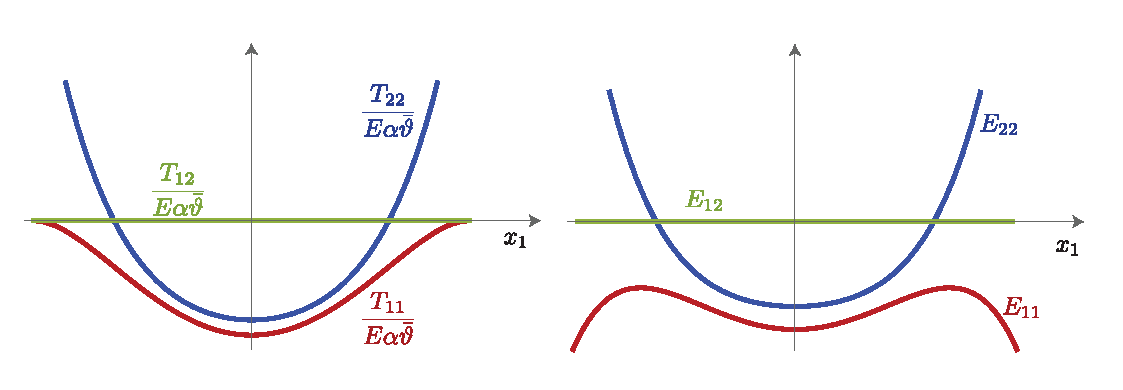
\includegraphics[scale=0.7]{figure/problema_elastico/rettangolo_termo}
\end{centering}


\end{svolgimento}
\end{exercise}

%
%\begin{remark}
%	L'equazione costitutiva inversa \eqref{constinvthe} consente in intuire se 
%	se in un corpo, completamente libero di deformarsi, s’instaurano delle tensioni in seguito a variazioni
%	termiche non uniformi. Decomponiamo la deformazione 
%	\begin{equation}
%		\Eb=\Eb^{\rm e}+\Eb^{\rm t}, \qquad \Eb^{\rm e}\coloneqq \Co^{-1}\Tb, \quad \Eb^{\rm t}\coloneqq \alpha(\vartheta-\vartheta_0)\,\Ib, 
%	\end{equation}
%	nella sua parte elastica e termica. Se le tensioni sono nulle
%	\begin{equation}
%		\Co(\Eb-\Eb^{\rm t})=\mathbf{0},
%	\end{equation}
%	ovvero, se il tensore di elasticità è definito positivo,
%	\begin{equation}
%		\Eb=\Eb^{\rm t}.
%	\end{equation}
%	Poiché
%	$
%	\Eb=\sym \nabla \ub
%	$,
%in ragione della  condizione di compatibilità \eqref{RotRot},	in un dominio semplicemente connesso $\Tb=\mathbf{0}$ se e solo se
%	\begin{equation}\label{rotrotEt}
%		\Rot \Rot \Eb^{\rm t}=\mathbf{0}.
%	\end{equation}
%	Se la variazione di temperatura è costante o lineare si ha che $\Eb^{\rm t}$  è costante e quindi la
%	\eqref{rotrotEt} è sicuramente verificata e per cui, in un corpo libero di deformarsi, non si crea stato di sforzo a seguito della variazione termica.
%	Non è difficile mostrare che la variazione lineare di temperatura è la condizione più  generale che non induce
%	uno stato tensionale.
%	
%	Intuitivamente possiamo pensare di dividere la configurazione di riferimento in regioni ``infinitesime'', in maniera che
%	si possa ritenere la temperatura costante su ciascuna regione infinitesima; in seguito alla variazione di temperatura, ogni regione infinitesima subirà
%	una deformazione $\Eb^{\rm t}=\alpha(\vartheta-\vartheta_0)$ dove, in prima approssimazione, $\vartheta-\vartheta_0$
%	rappresenta la media di $(\vartheta-\vartheta_0)(\xb)$ sulla regione infinitesima. Una volta deformate le singole regioni, a causa di $\Eb^{\rm t}$, si devono riassemblare: se è 
%	possibile farlo senza doverle ulteriormente deformare non s’instaura della tensione,
%	se invece regioni infinitesime confinanti non si riescono a riassemblare in
%	maniera continua si dovrà produrre una deformazione $\Eb^{\rm e}$ per ripristinare la
%	continuità, e quindi introdurre una tensione $\Tb=\Co \Eb^{\rm e} $.
%	
%\end{remark}





%
%\subsection{Problemi in coordinate polari}
%
%In coordinate polari il pi\`{u} generico stato di sforzo autoequilibrato pu\`{o} porsi nella forma:
%\begin{equation}\label{Airy_polare}
%	\begin{aligned}
%		T_\rho&=\frac{1}{\rho}\varphi,_r+\frac{1}{\rho^2}\varphi,_{\vartheta \vartheta} \\[1mm]
%		T_{\vartheta}&=\varphi,_{\rho \rho}\\[1mm]
%		T_{\rho\vartheta}&=\frac{1}{\rho^2}\varphi,_{\vartheta} -\frac{1}{\rho}\varphi,_{\vartheta \rho} 
%	\end{aligned}
%\end{equation}
%dove $\varphi=\varphi(\rho,\, \vartheta)$ \`{e} la funzione di Airy. Questo soddisfa le condizioni di compatibilit\`{a} cinematica se risulta:
%\begin{equation}\label{Stati_piani_cil_01}
%	\left(\partial_{\rho\rho}+\frac{1}{\rho}\partial_\rho+\frac{1}{\rho^2}\partial_{\vartheta \vartheta}\right)\left(\partial_{\rho\rho}\varphi+\frac{1}{\rho}\partial_\rho\varphi+\frac{1}{\rho^2}\partial_{\vartheta \vartheta}\varphi\right)=0
%\end{equation} 
%ovvero $\Delta\Delta\varphi=0$.
%
%%
%Si esaminano le soluzioni di alcuni problemi di bordo le cui soluzioni tensionali prescindono dal legame costitutivo. Poich\'{e} queste riguardano problemi di rilevante interesse ingegneristico sia in regime piano di deformazione sia di tensione, le soluzioni sono espresse in termini di tensioni puntuali e non generalizzate. Esse, pertanto, coincidono con quelle effettive dello stato di deformazione piano mentre forniscono una stima dei valori medi nello spessore per lo stato piano di tensione.
%
%
%\subsubsection{La soluzione di Michell}
%Cerchiamo una soluzione generale dell'equazione di Airy assumendo che abbia una forma a variabili separabili:
%\begin{equation}
%\varphi(\rho, \vartheta)=f(\rho)e^{\beta \vartheta},
%\end{equation}
%dove la costante $\beta$ è un parametro da determinare. Sostituendo nell'equazione biarmonica e cancellando il termine comune $e^{\beta \vartheta}$ si ottiene
%\begin{equation}
%f^{''''}(\rho)+\frac{2}{\rho}\,f'''(\rho)-\frac{1-2\beta^2}{\rho^2}\,f''(\rho)+\frac{1-2\beta^2}{\rho^3}\,f'(\rho)+\frac{\beta^2(4+\beta^2)}{\rho^3}\, f(\rho)=0.
%\end{equation}
%
%Per risolvere questa equazione,  effettuiamo un cambio di variabile
%\begin{equation}
%\rho=e^{\xi}, \qquad f(\rho)=\hat{f}(\xi),
%\end{equation}
%per ottenere
%\begin{equation}
%\hat{f}''''(\xi)-f'''(\xi)+(4+2b^2)\hat{f}''(\xi)-4b^2\hat{f}'(\xi)+b^2(4+b^2)\hat{f}(\xi)=0.
%\end{equation}
%La soluzione di questa equazione si può trovare usando la solita tecnica, cercando
%\begin{equation}
%\hat{f}(\xi)=e^{\alpha \xi},
%\end{equation}
%che dà luogo alla seguente equazione caratteristica:
%\begin{equation}
%(\alpha^2+\beta^2)(\alpha^2-4\alpha+4+\beta^2)=0,
%\end{equation}
%le cui radici sono
%\begin{equation}
%	\alpha=\pm i \beta, \quad \alpha=2\pm i \beta
%\end{equation}
%oppure
%\begin{equation}
%\beta=\pm i \alpha, \quad \beta=\pm i(\alpha-2).
%\end{equation}
%
%Considereremo solo soluzioni periodiche in $\vartheta$, che si ottengono scegliendo $\beta=in$, con $n\in \mathbb{Z}$. Questa scelta implica che anche $\alpha$ sia un intero. Per particolai valori di $n$ alcune radici sono ripetute ed occorrono speciali considerazioni nello sviluppo della soluzione.
%
%
%Le soluzioni periodiche in $\vartheta$ dell'equazione di Airy 
%sono state determinate da Michell nel 1899. La loro espressione è:
%\begin{equation}
%	\begin{aligned}
%		\varphi &= a_0 + a_1\log \rho+a_2~\rho^2 +a_3~\rho^2 \log \rho \\
%		& + \left(a_4+a_4\log \rho+a_6~\rho^2+a_7~\rho^2\log \rho\right) \vartheta \\
%		& + \left(a_{11}~\rho +a_{12}~\rho\log \rho+\frac{a_{13}}{\rho}+a_{14}~\rho^3+a_{15}~\rho\vartheta+a_{16} ~\rho\vartheta\log \rho  \right) \cos\vartheta \\
%		& + \left(b_{11}~\rho +b_{12}~\rho\log \rho+\frac{b_{13}}{\rho}+a_{14}~\rho^3+b_{15}~\rho\vartheta+b_{16} ~\rho\vartheta\log \rho \right) \sin\vartheta \\
%		& + \sum_{n=2}^{\infty} \left(a_{1}~\rho^n + a_{n2}~\rho^{2+n} + a_{n3}~\rho^{-n} + a_{4}~\rho^{2-n}\right)\cos(n\vartheta) \\
%		& + \sum_{n=2}^{\infty} \left(b_{1}~\rho^n + b_{n2}~\rho^{2+n} + b_{n3}~\rho^{-n} + b_{4}~\rho^{2-n}\right)\sin(n\vartheta)\,,
%	\end{aligned}
%\end{equation}
%dove $a_n$, $a_{nm}$ a $b_{nm}$ sono costanti da determinare. 
%
%Nel caso assialsimetrico, i campi sono indipendenti dalla coordinata $\vartheta$ e dunque la soluzione di Michell si riduce a 
%\begin{equation}
%\varphi=a_0+a_1\log r+a_2 \rho^2+a_3\log \rho.
%\end{equation}
%Le corrispondenti componenti di sforzo risultano essere:
%\begin{align}\label{tenspolar}
%	&T_\rho=2 a_3\log \rho+\frac{a_1}{\rho^2}+a_3+2a_2,\\
%	&T_\vartheta=2 a_3\log \rho-\frac{a_1}{\rho^2}+3a_3+2a_2,\\
%	&T_{\rho\vartheta}=0.
%\end{align}
%Integrando la relazione deformazioni-spostamenti, si trovano le componenti di spostamento:
%\begin{align}
%	&u_\rho=\frac{1}{E}\left[  -\frac{1+\nu}{\rho}\,a_1+2(1-\nu)a_3 \rho\log \rho-(1+\nu)a_3 \rho+2a_2(1-\nu)\rho  \right]+A\sin\vartheta+B\cos\vartheta,\\
%	&u_\vartheta=\frac{4\rho\vartheta}{a_3}+A\cos\vartheta-B\sin\vartheta+C\rho,\label{ua}
%\end{align}
%dove $A$, $B$ e $C$ sono costanti abitrarie associate al moto rigido. Se il dominio inlcude l'origine, allora $a_3$ e $a_1$ devono essere nulli in modo da mantenere finite le tensioni. In tal caso, lo sforzo è costante. Inoltre il termine che moltiplica $a_3$ in \eqref{ua} è una funzione polidroma se la geometria del dominio è tale da includere l'origine tramite una curva chiusa omotopa a zero.
%
%
%Vediamo alcune soluzioni di interesse.
%
%\vspace{.5cm}
%
%\noindent\textsf{\small\textit{\textbf{Cilindro cavo con pressione al bordo}}}
%
%Il primo esempio che verrà analizzato riguarda un cilindro cavo a parete spessa sottoposto all'azione di pressioni interne ed esterne uniformi, come mostrato nella Figura \ref{label}. Si assume che il cilindro sia lungo e che questo problema possa essere modellato in condizioni di deformazione piana.
%
%Utilizzando la soluzione delle tensioni \eqref{tenspolar} senza i termini logaritmici, le tensioni non nulle sono date da
%
%\begin{equation}
%T_\rho = \frac{A}{\rho^2} + B, \qquad T_{\vartheta}= -\frac{A}{\rho^2} + B
%\end{equation}
%Applicando le condizioni al contorno \(T_\rho(\rho_1) = -p_1\), \(T_\rho(\rho_2) = -p_2\), si ottengono due equazioni per le due costanti incognite \(A\) e \(B\). Risolvendo per queste costanti si ottiene il risultato
%
%\[
%A = \frac{\rho_1^2 \rho_2^2 (p_2 - p_1)}{\rho_2^2 - \rho_1^2} \quad \text{(8.4.2)}
%\]
%\[
%B = \frac{\rho_2^2 p_1 - \rho_1^2 p_2}{\rho_2^2 - \rho_1^2}
%\]
%
%Sostituendo questi valori nella relazione (8.4.1), si ottiene la forma finale del campo di tensioni:
%
%\[
%T_\rho = \frac{\rho_1^2 \rho_2^2 (p_2 - p_1)}{\rho_2^2 - \rho_1^2} \frac{1}{\rho^2} + \frac{\rho_1^2 p_1 - \rho_2^2 p_2}{\rho_2^2 - \rho_1^2} \quad 
%\]
%\[
%T_\theta = -\frac{\rho_1^2 \rho_2^2 (p_2 - p_1)}{\rho_2^2 - \rho_1^2} \frac{1}{\rho^2} + \frac{\rho_1^2 p_1 - \rho_2^2 p_2}{\rho_2^2 - \rho_1^2}
%\]
%
%
%Dalla teoria della deformazione piana, la tensione longitudinale fuori dal piano è data da
%
%\[
%T_z = \nu (T_\rho + T_\theta) = 2\nu \frac{\rho_1^2 p_1 - \rho_2^2 p_2}{\rho_2^2 - \rho_1^2} 
%\]
%
%Utilizzando le relazioni di spostamento-deformazione \eqref{} e la legge di Hooke \eqref{}), lo spostamento radiale si determina facilmente come
%
%\[
%u_\rho = \frac{1+\nu}{E} \rho \left[ (1 - 2\nu) B - \frac{A}{\rho^2} \right]
%\]
%\[
%= \frac{1+\nu}{E} \left[ - \frac{\rho_1^2 \rho_2^2 (p_2 - p_1)}{\rho_2^2 - \rho_1^2} \frac{1}{\rho} + (1 - 2\nu) \frac{\rho_1^2 p_1 - \rho_2^2 p_2}{\rho_2^2 - \rho_1^2} \rho \right]  
%\]
%
%Esaminando questa soluzione, si nota che per il problema con condizioni al contorno di trazione e senza forze di corpo, il campo di tensioni non dipende dalle costanti elastiche. Tuttavia, gli spostamenti risultanti dipendono sia da \(E\) che da \(\nu\).
%
%Nel caso di sola pressione interna (\(p_2 = 0\) e \(p_1 = p\)) con \(\rho_1 / \rho_2 = 1/2\), la distribuzione non dimensionalizzata delle tensioni attraverso lo spessore della parete è mostrata in Figura \ref{8-9}. La tensione radiale decade da \(-p\) a zero, mentre la tensione circonferenziale è sempre positiva con un valore massimo al raggio interno \((\sigma_\theta)_{\text{max}} = \frac{r_1^2 + r_2^2}{r_2^2 - r_1^2} p = \frac{5}{3} p\).
%
%Nel caso di un tubo a parete sottile, si può dimostrare che la tensione circonferenziale si riduce alla ben nota relazione della teoria della resistenza dei materiali:
%
%\[
%\sigma_\theta \approx \frac{p r_0}{t} \quad \text{(8.4.6)}
%\]
%
%dove \(t = r_2 - r_1\) è lo spessore e \(r_0 = (r_1 + r_2) / 2\) è il raggio medio.
%
%La soluzione generale per questo esempio può essere utilizzata per generare la soluzione ad altri problemi attraverso semplici processi di scalatura. Tali casi sono ora presentati.
%





